% Supplementary qualitative pages (rendered by paper/figures/make_supp_qual.py). Needs macros.tex.

\begin{figure*}[p]
\centering
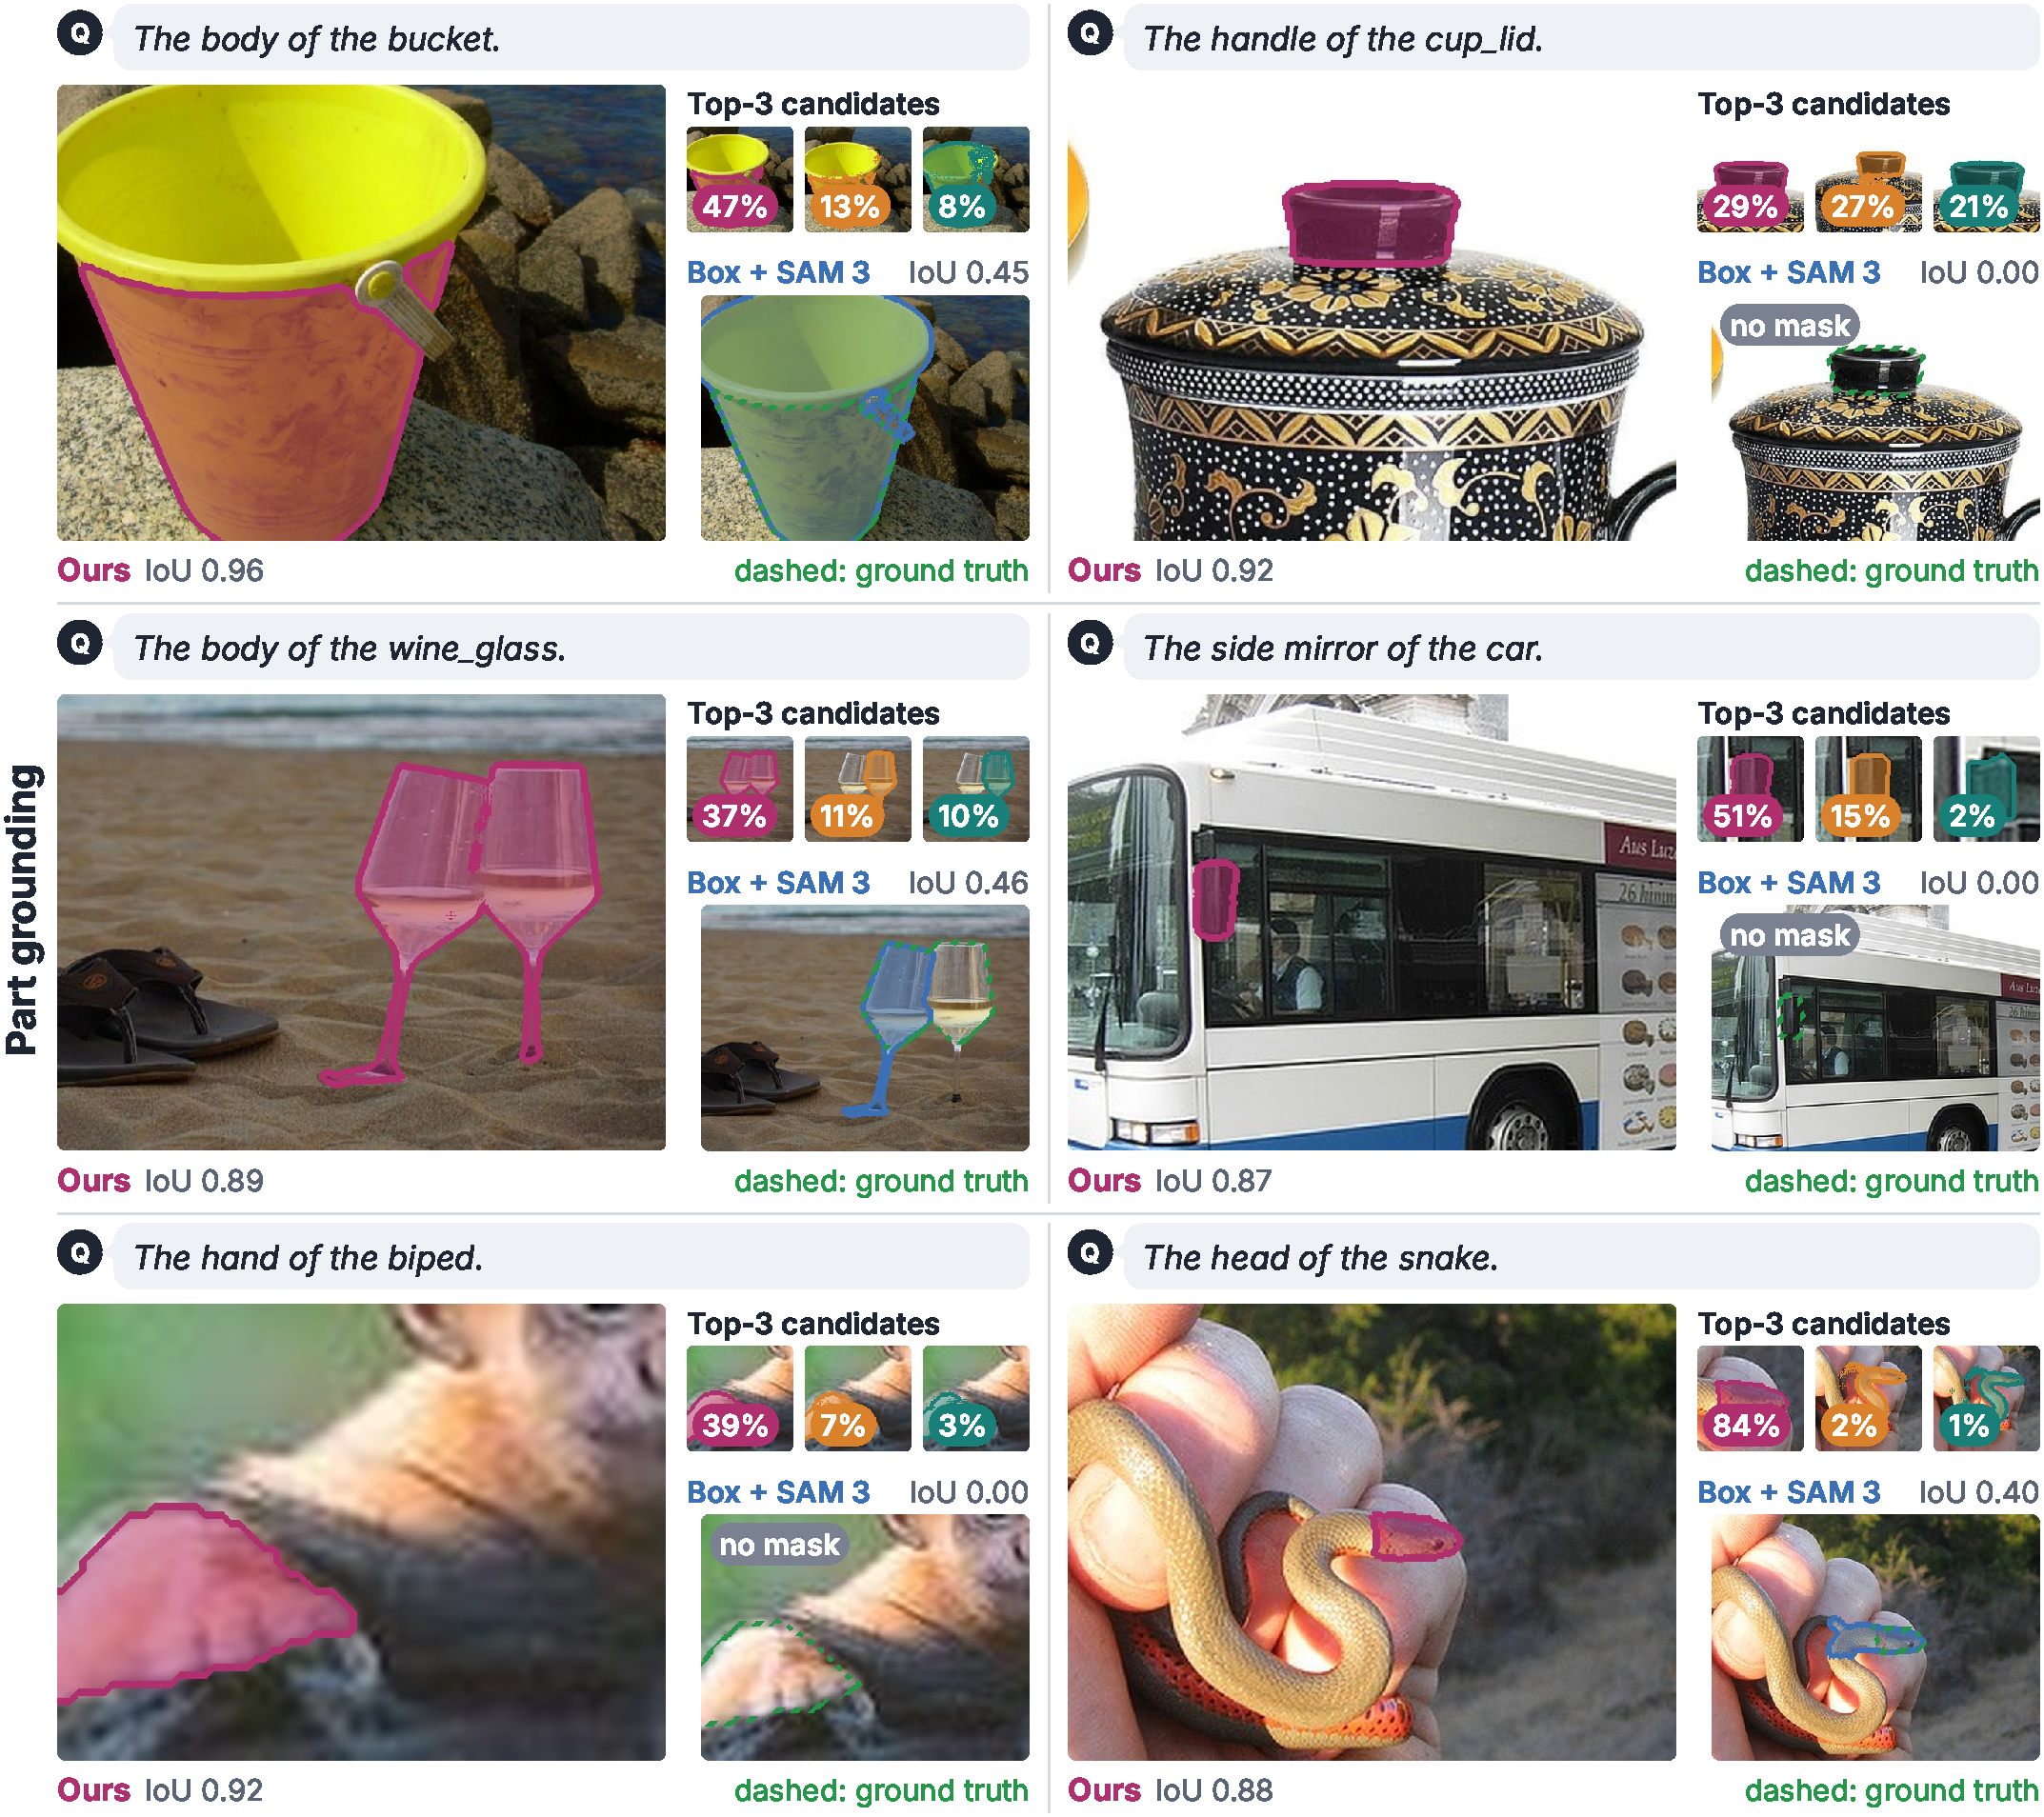
\includegraphics[width=\textwidth,height=0.9\textheight,keepaspectratio]{figures/qualitative/supp/part_selected_1.pdf}
\caption{\textbf{Part grounding: selected examples (1/3).} Test examples where \ours{} clearly beats Box + SAM\,3, in the format of Fig.~\ref{fig:showcase}; none of them appears in the main paper. Filled magenta: the mask \ours{} selects; blue: baselines; dashed green: ground truth.}
\label{fig:supp_part_selected_1}
\end{figure*}

\begin{figure*}[p]
\centering
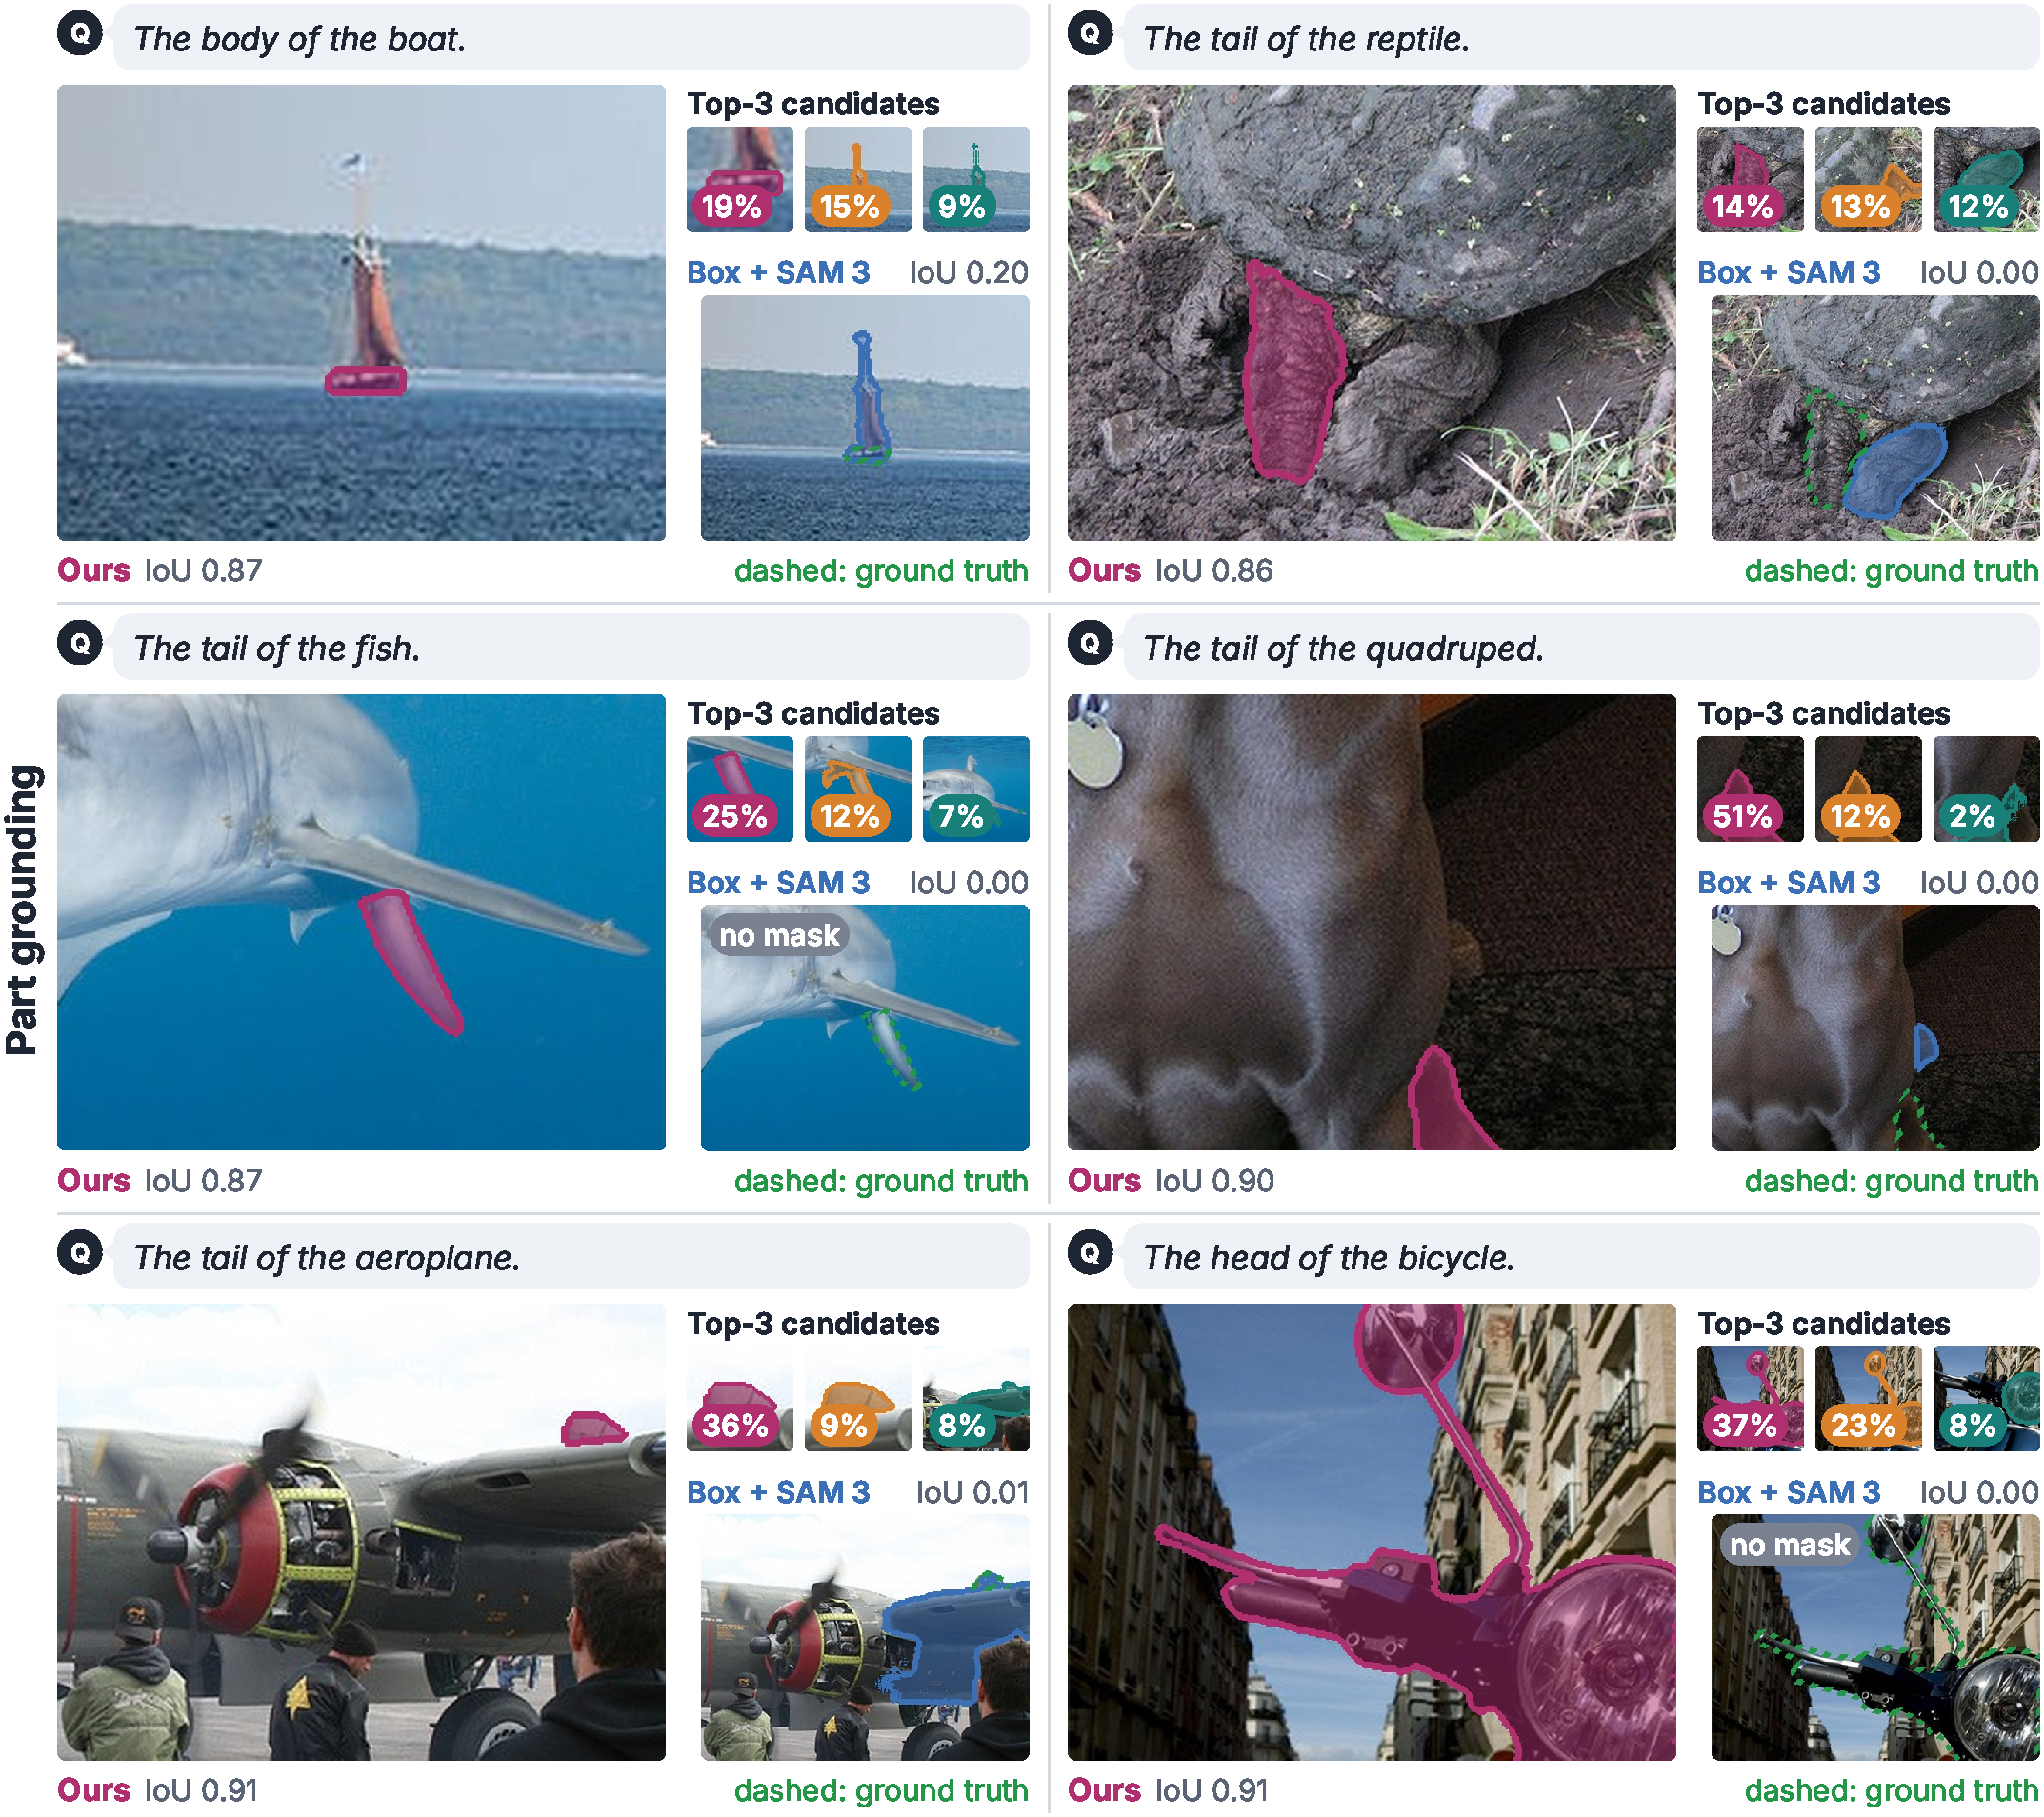
\includegraphics[width=\textwidth,height=0.9\textheight,keepaspectratio]{figures/qualitative/supp/part_selected_2.pdf}
\caption{\textbf{Part grounding: selected examples (2/3).} Test examples where \ours{} clearly beats Box + SAM\,3, in the format of Fig.~\ref{fig:showcase}; none of them appears in the main paper. Filled magenta: the mask \ours{} selects; blue: baselines; dashed green: ground truth.}
\label{fig:supp_part_selected_2}
\end{figure*}

\begin{figure*}[p]
\centering
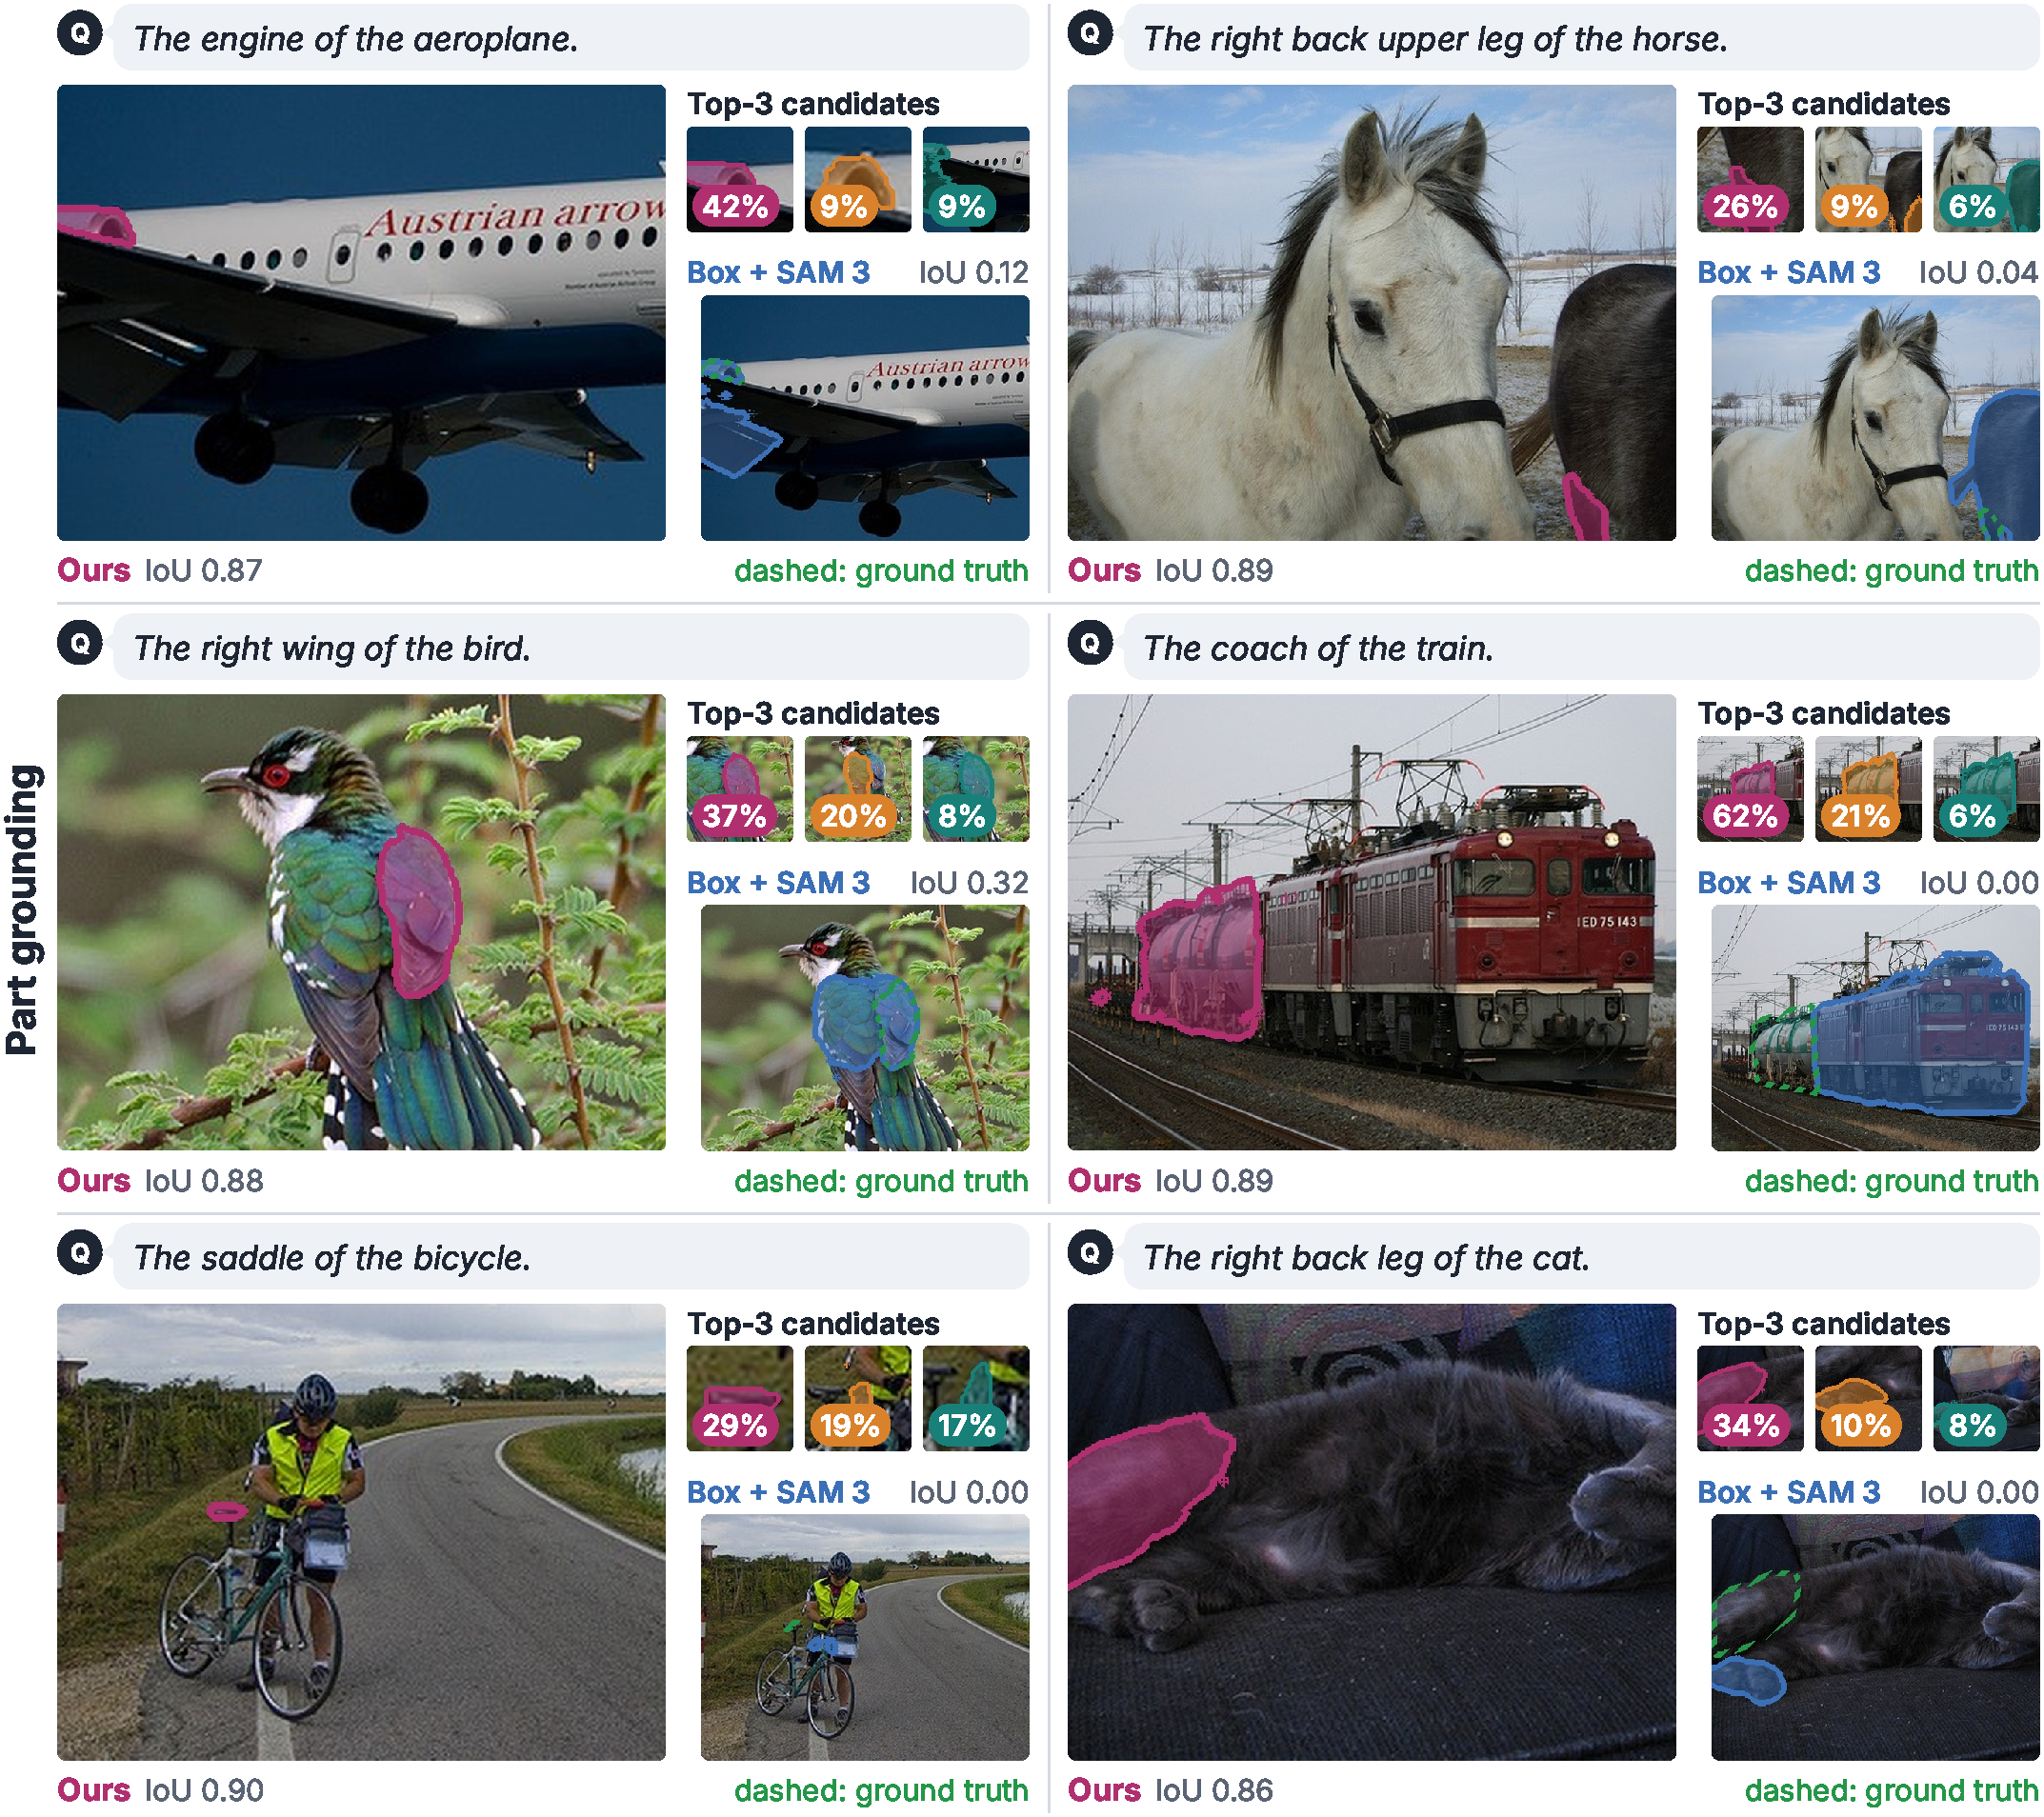
\includegraphics[width=\textwidth,height=0.9\textheight,keepaspectratio]{figures/qualitative/supp/part_selected_3.pdf}
\caption{\textbf{Part grounding: selected examples (3/3).} Test examples where \ours{} clearly beats Box + SAM\,3, in the format of Fig.~\ref{fig:showcase}; none of them appears in the main paper. Filled magenta: the mask \ours{} selects; blue: baselines; dashed green: ground truth.}
\label{fig:supp_part_selected_3}
\end{figure*}

\begin{figure*}[p]
\centering
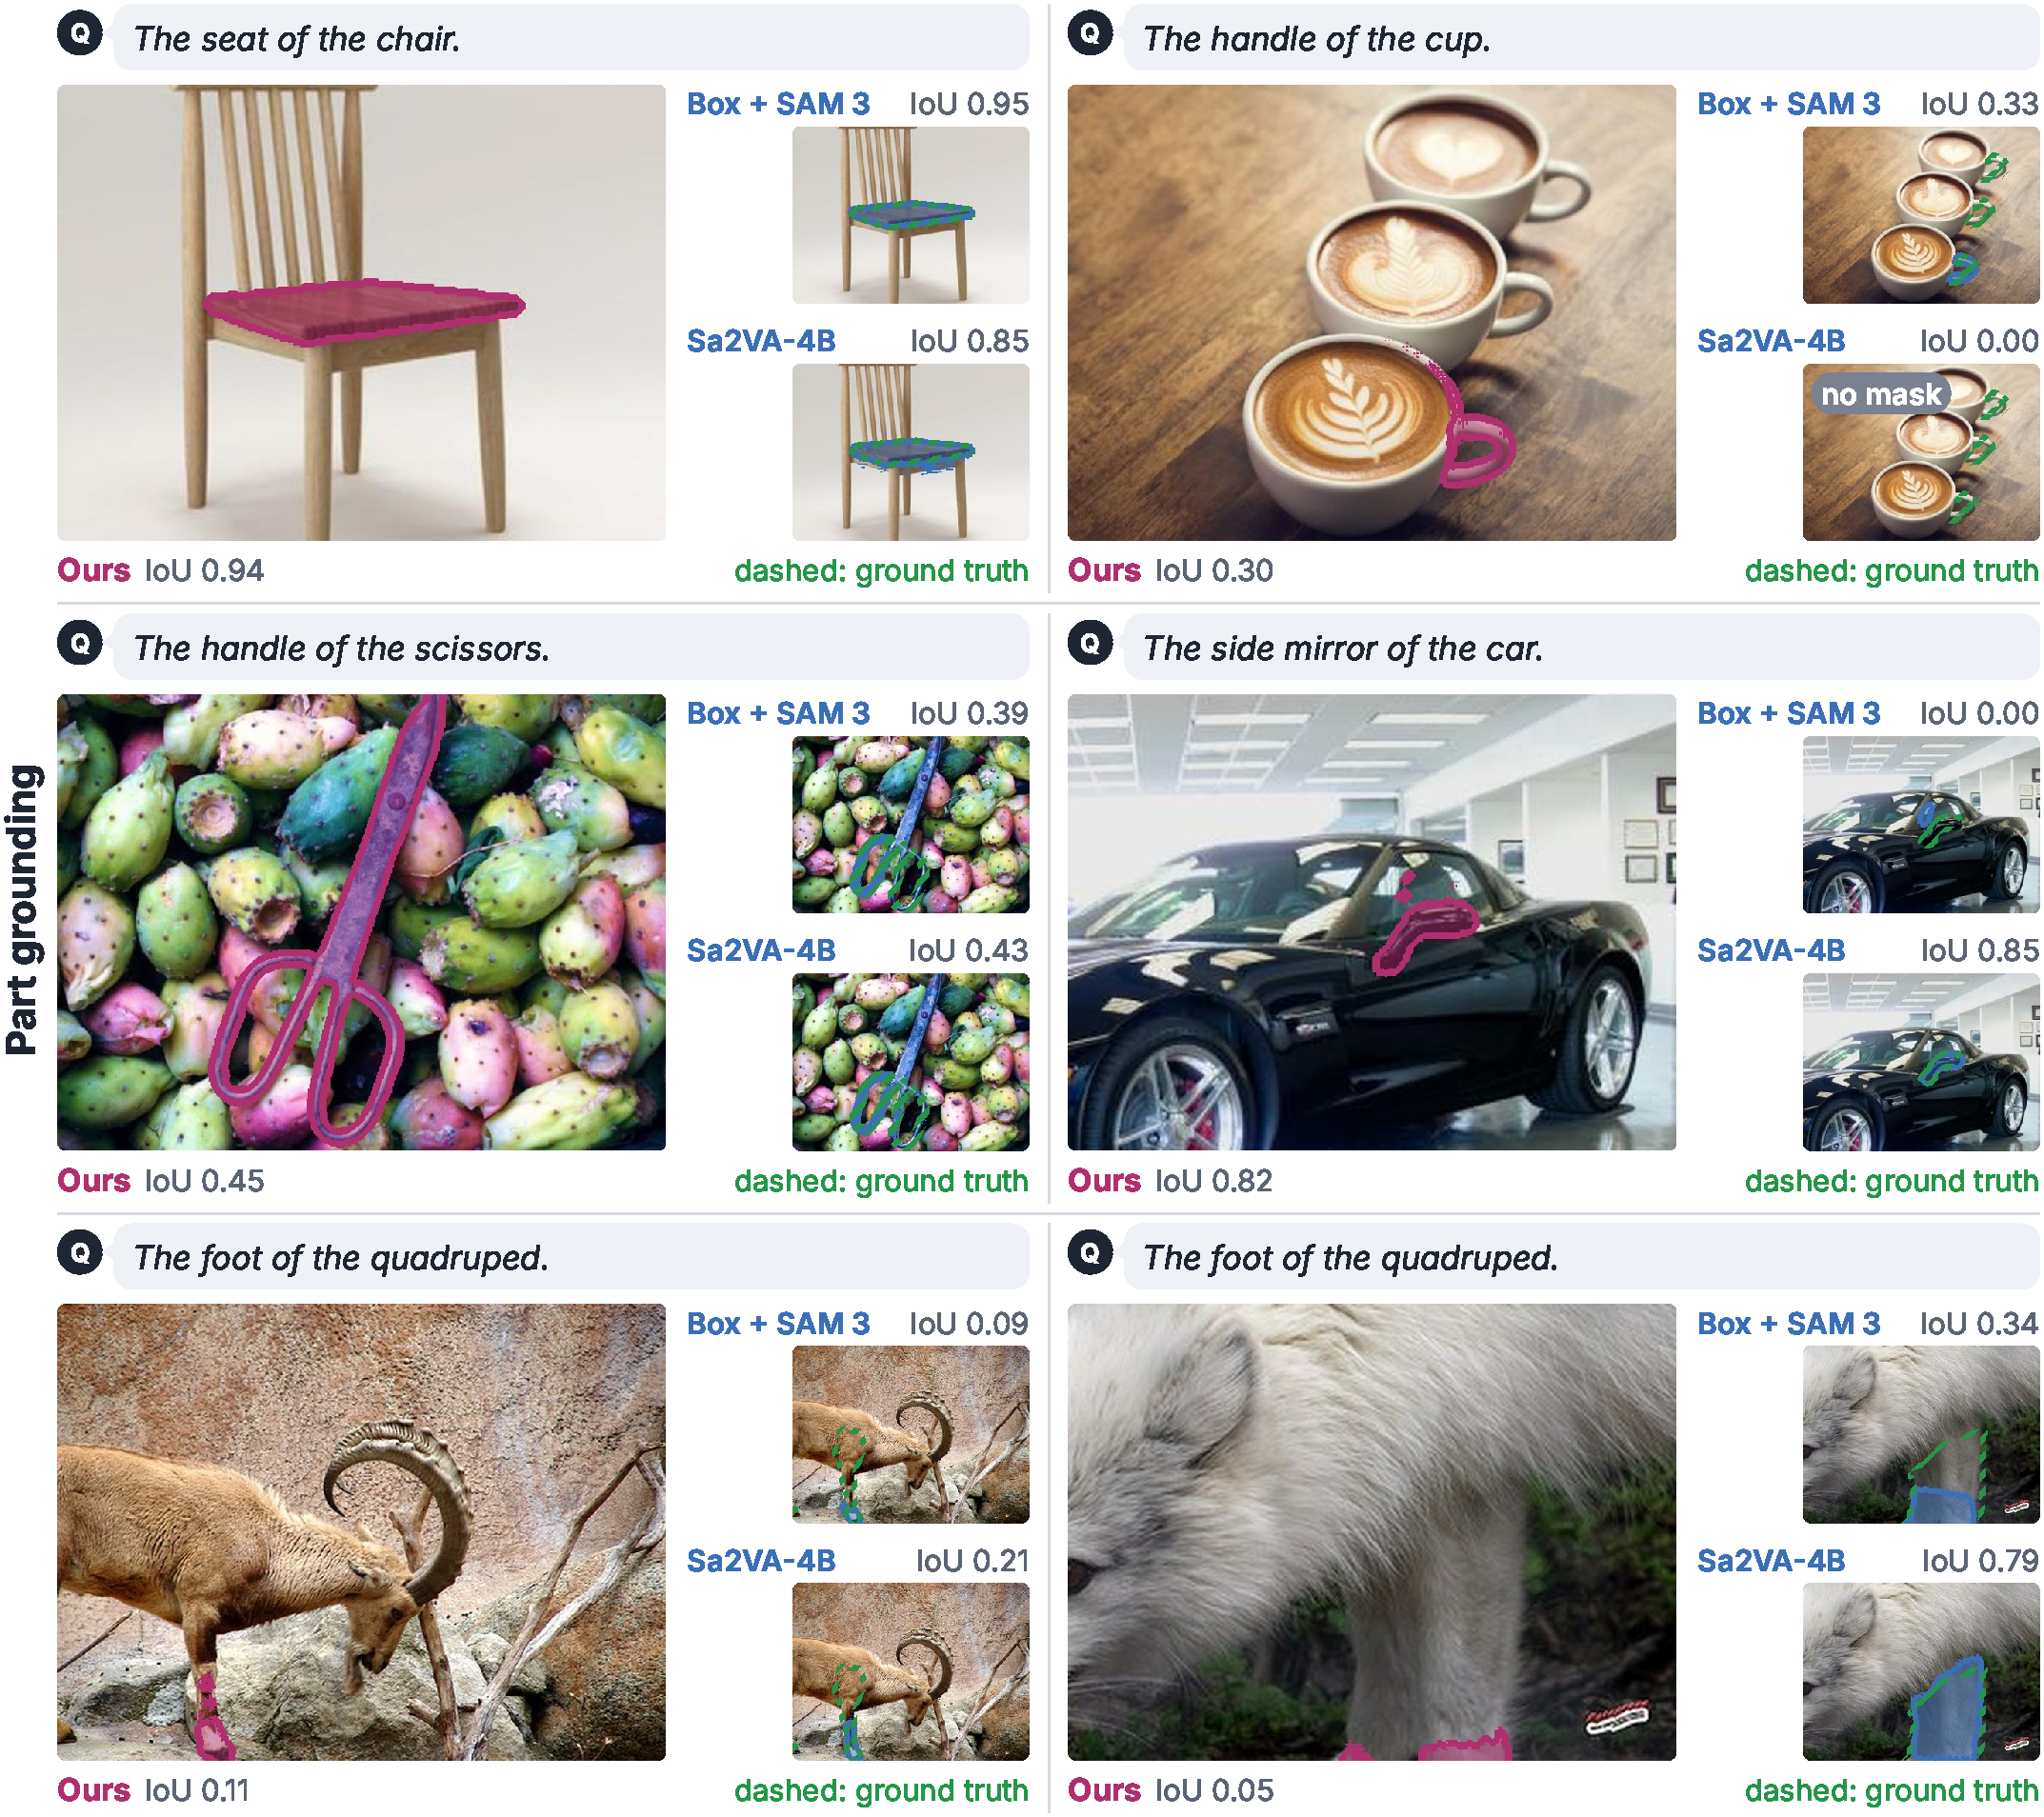
\includegraphics[width=\textwidth,height=0.9\textheight,keepaspectratio]{figures/qualitative/supp/part_random.pdf}
\caption{\textbf{Part grounding: random examples.} A fixed-seed random sample of test queries, not selected for outcome. Filled magenta: the mask \ours{} selects; blue: baselines; dashed green: ground truth.}
\label{fig:supp_part_random}
\end{figure*}

\begin{figure*}[p]
\centering
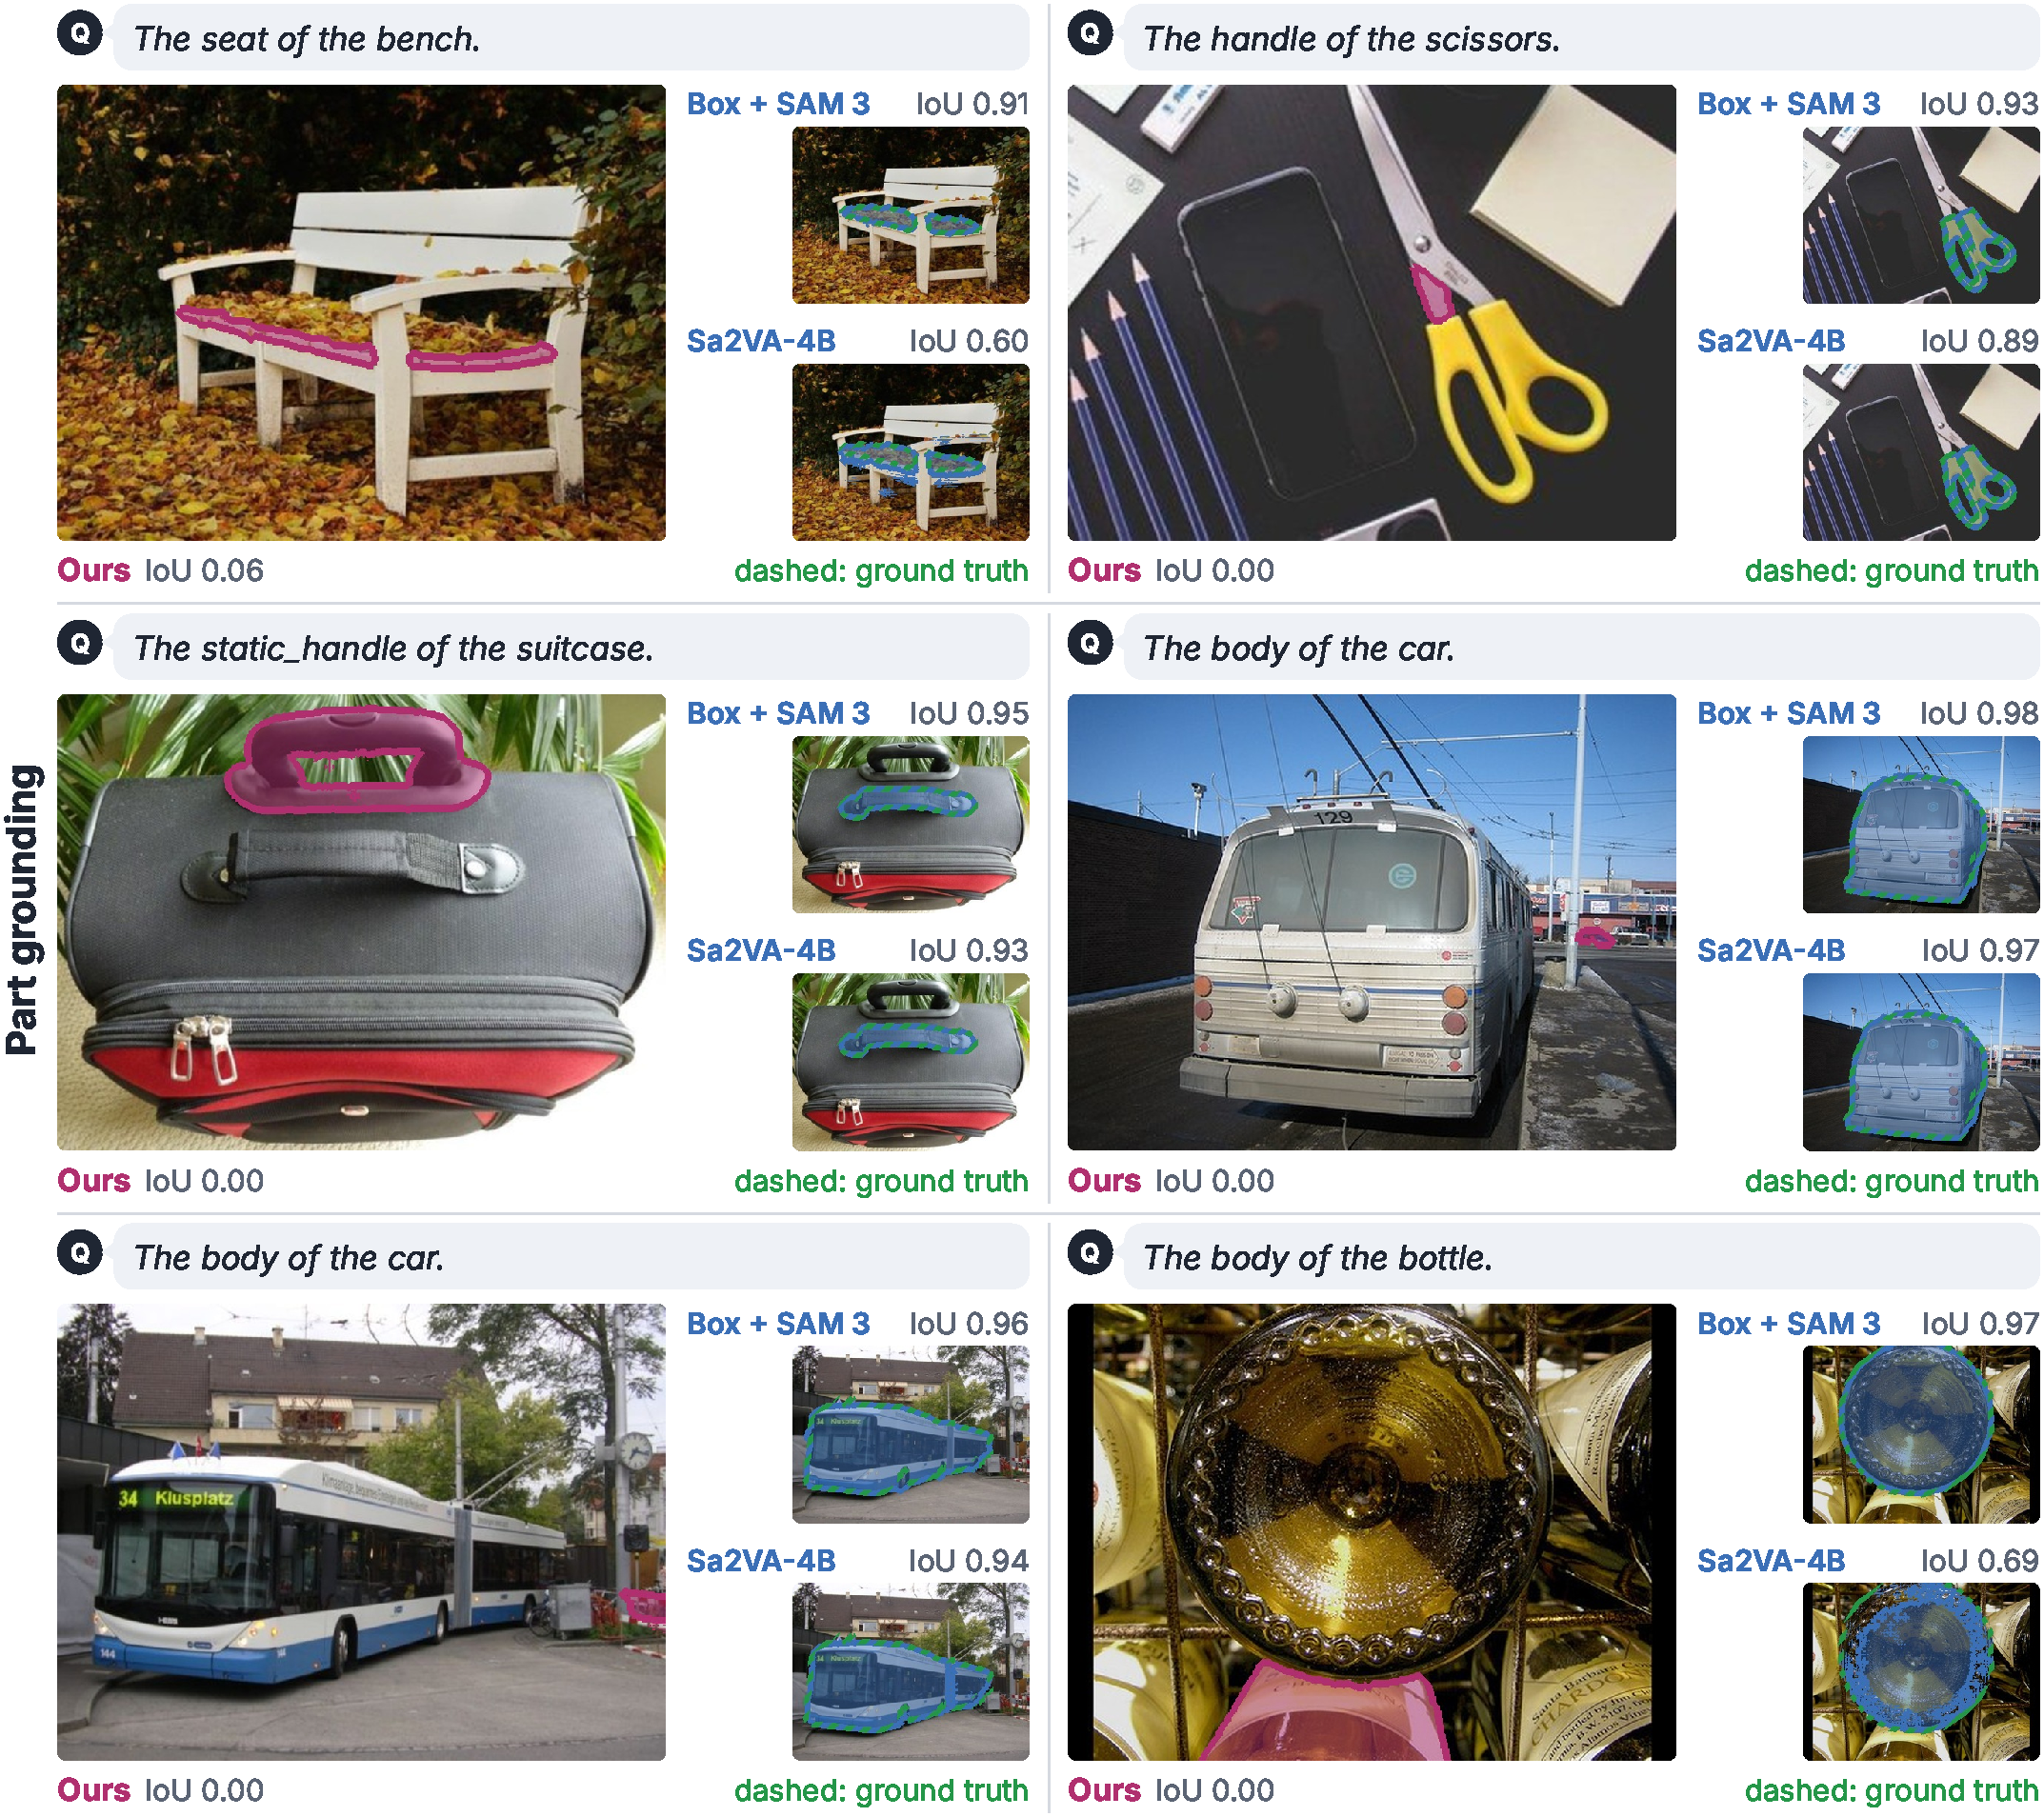
\includegraphics[width=\textwidth,height=0.9\textheight,keepaspectratio]{figures/qualitative/supp/part_failures.pdf}
\caption{\textbf{Part grounding: failure cases.} The test queries where \ours{} falls furthest behind Box + SAM\,3. Filled magenta: the mask \ours{} selects; blue: baselines; dashed green: ground truth.}
\label{fig:supp_part_failures}
\end{figure*}

\begin{figure*}[p]
\centering
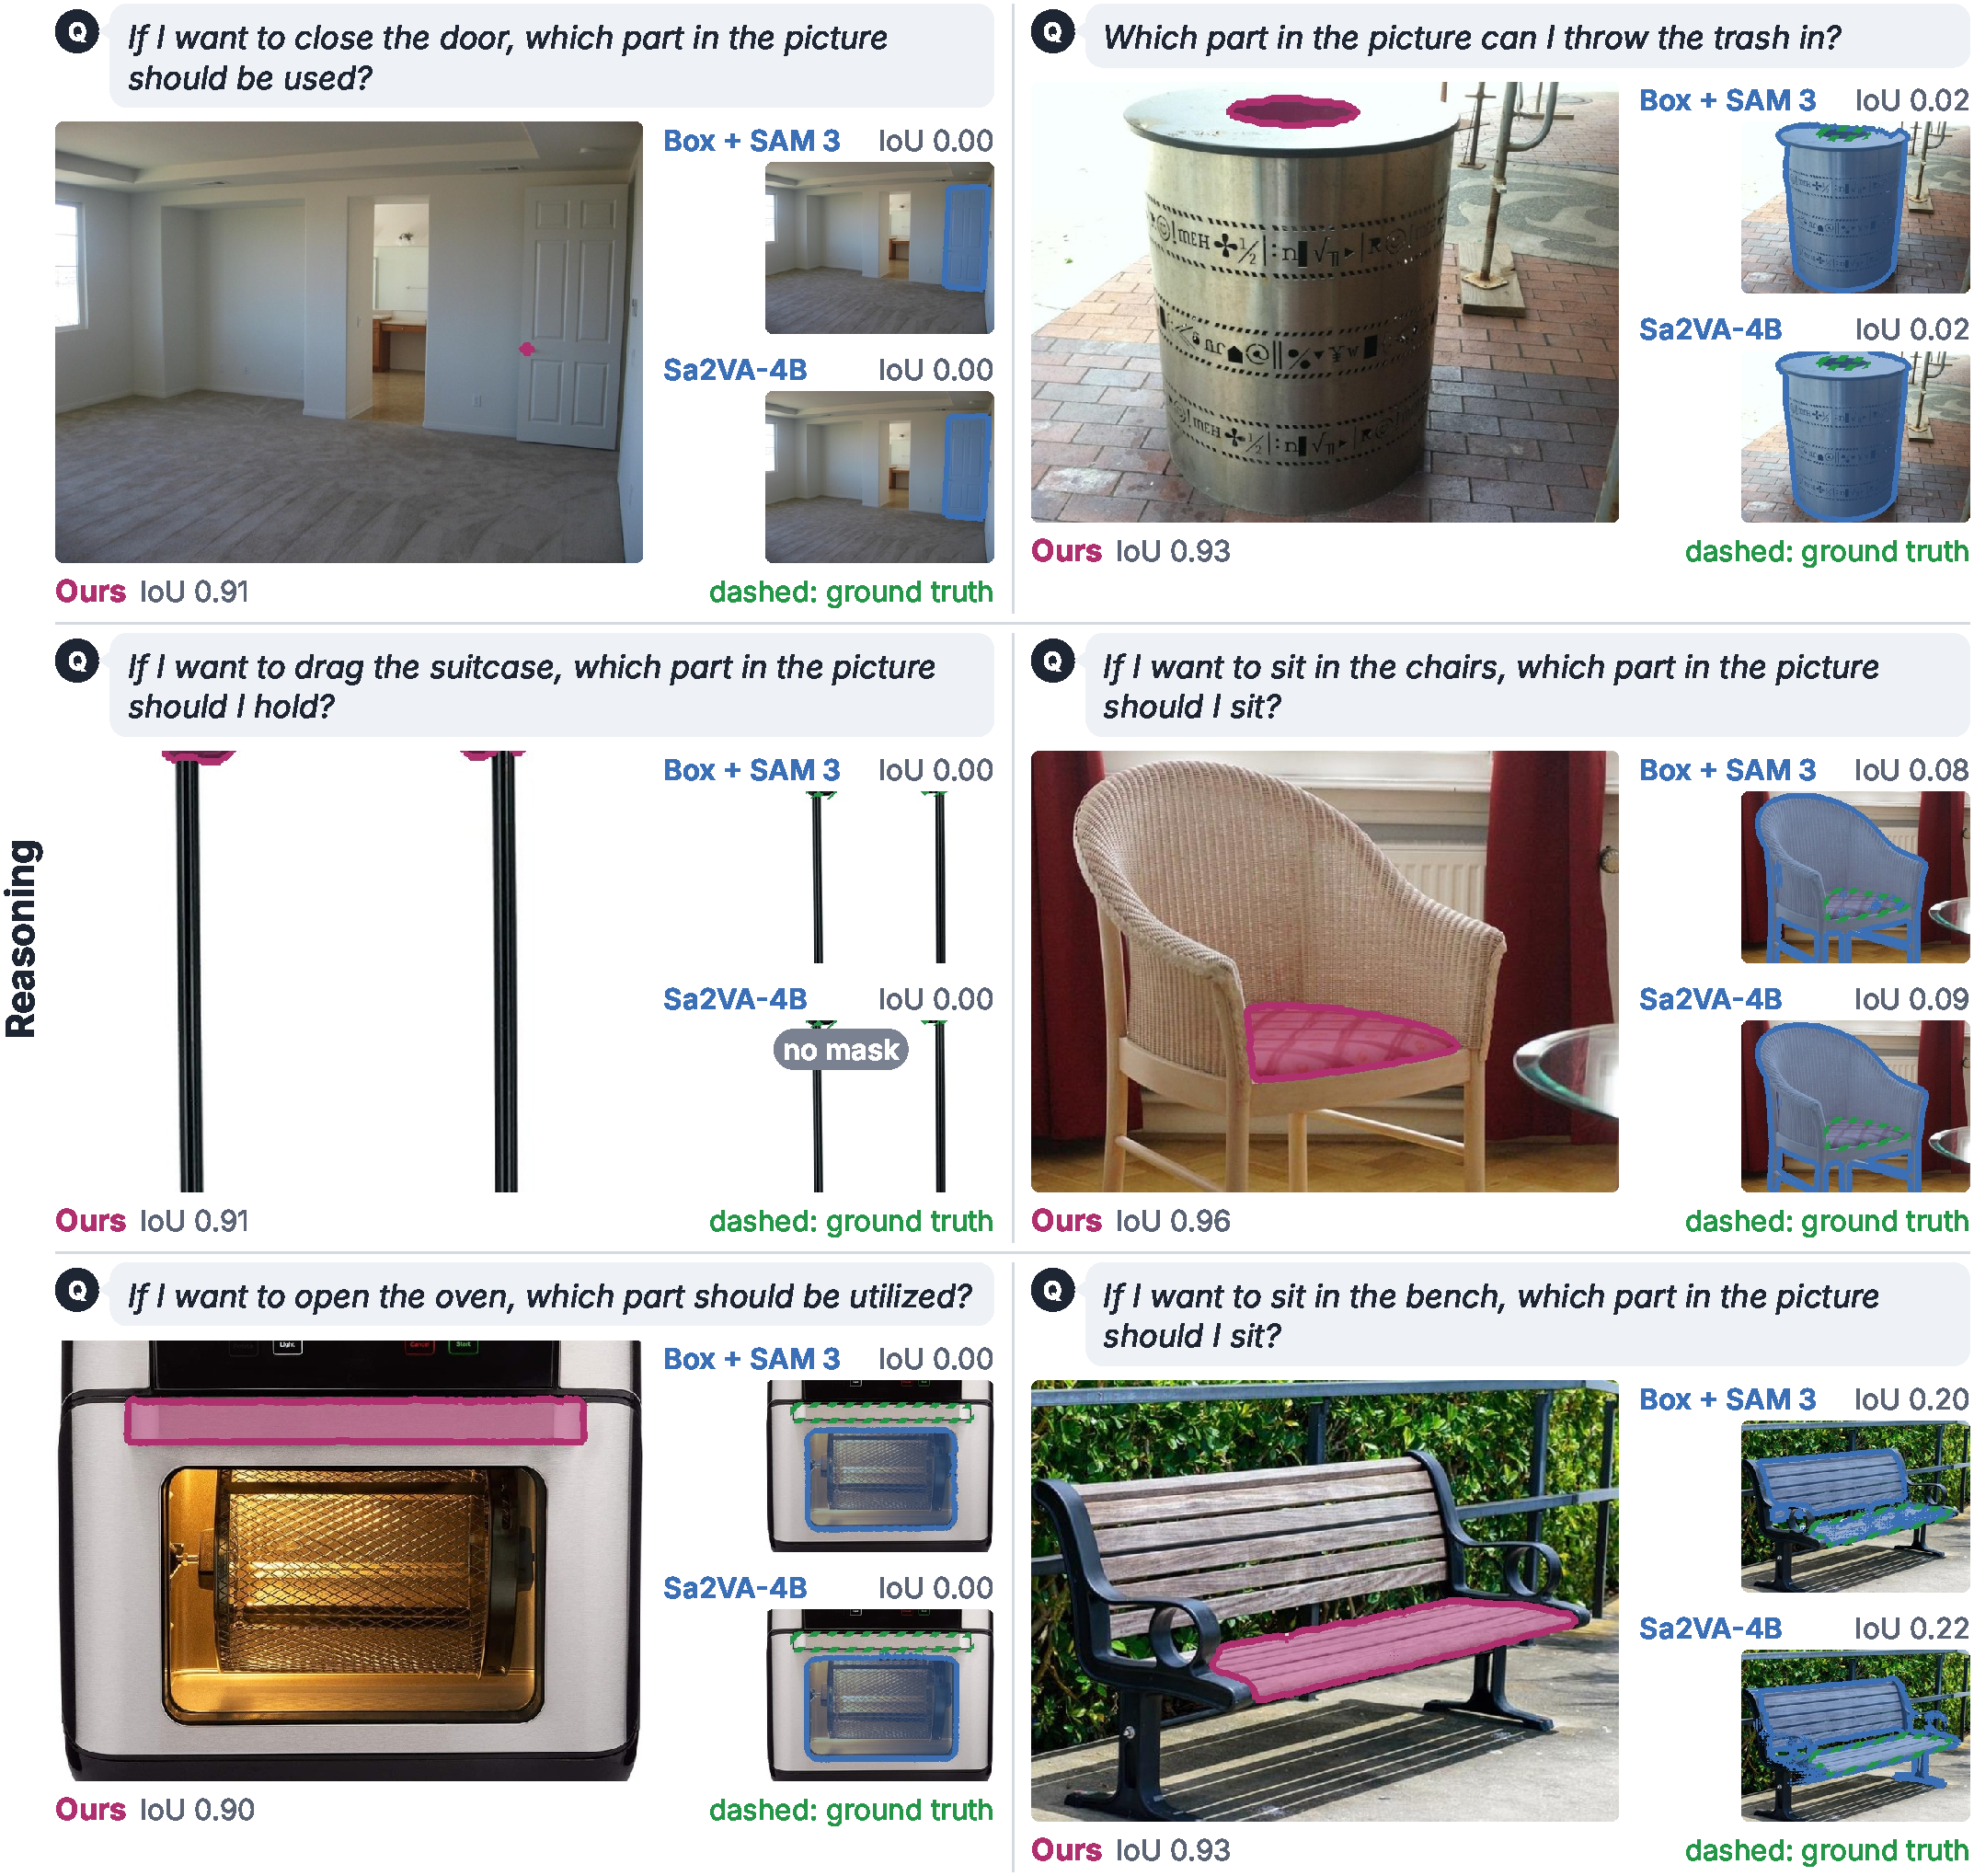
\includegraphics[width=\textwidth,height=0.9\textheight,keepaspectratio]{figures/qualitative/supp/reason_selected_1.pdf}
\caption{\textbf{Reasoning: selected examples (1/3).} Test examples where \ours{} clearly beats Box + SAM\,3, in the format of Fig.~\ref{fig:showcase}; none of them appears in the main paper. Selected examples use query rewriting; random examples and failure cases show \ours{} without it.}
\label{fig:supp_reason_selected_1}
\end{figure*}

\begin{figure*}[p]
\centering
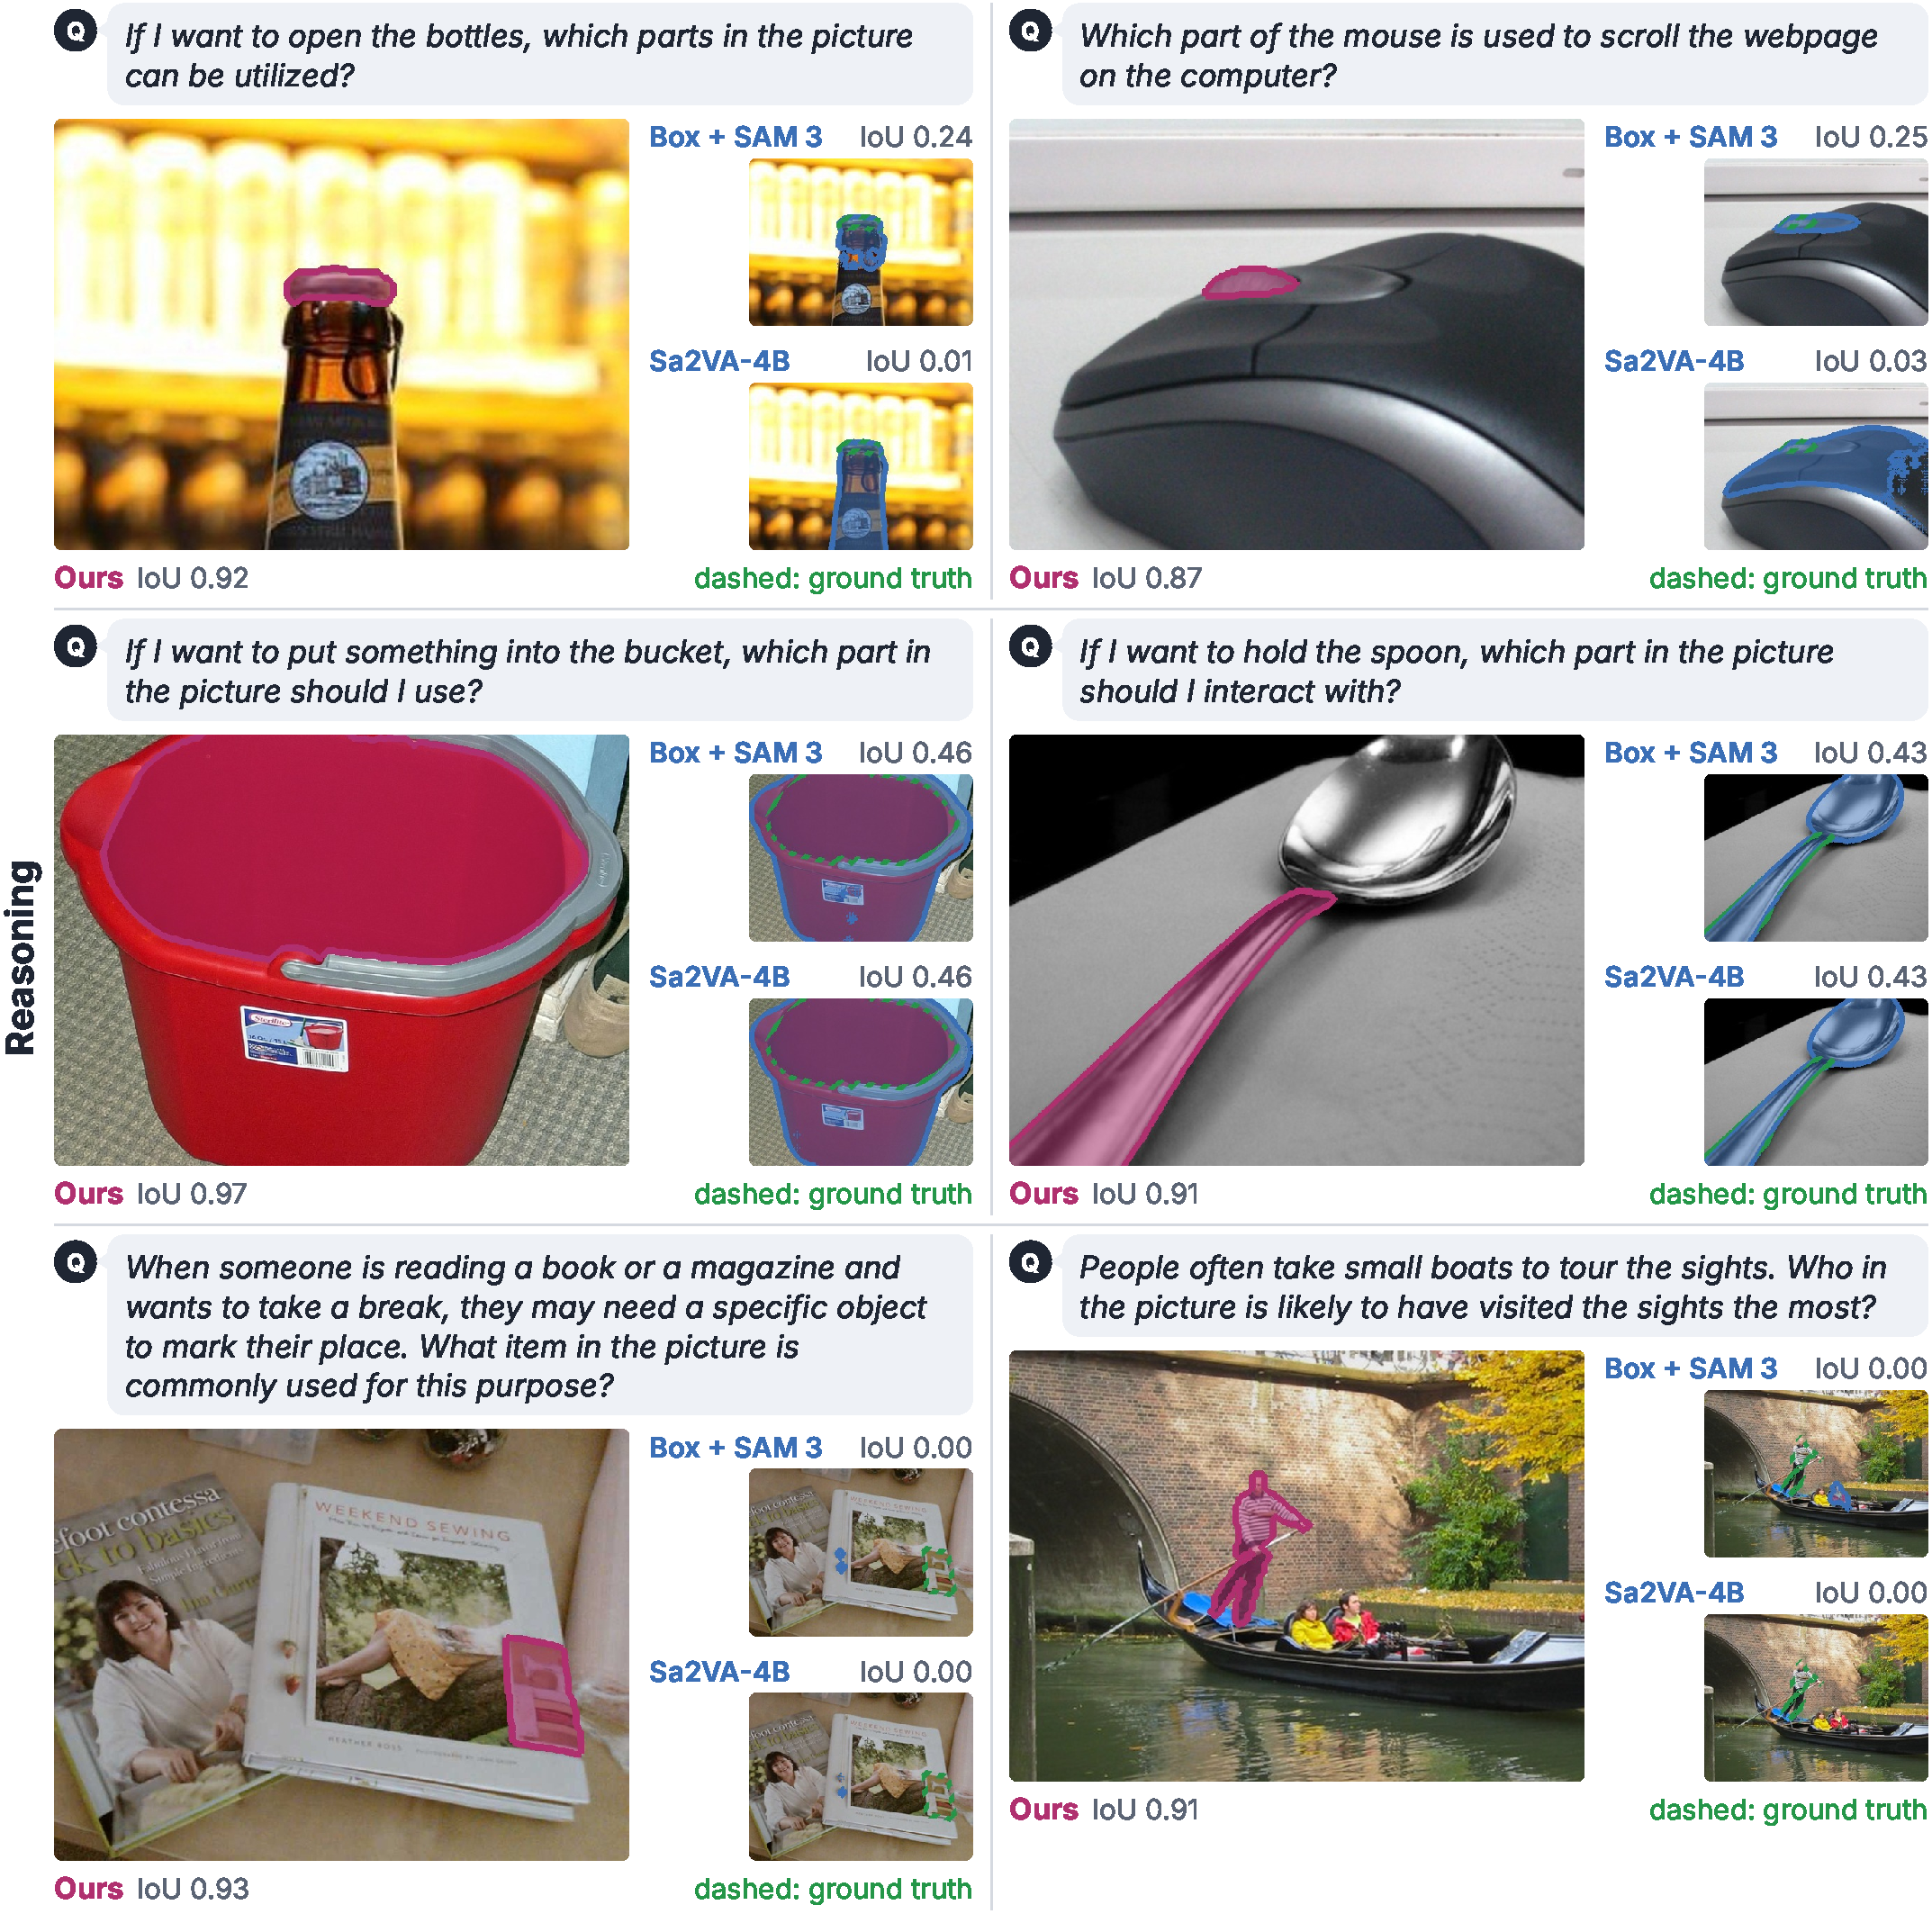
\includegraphics[width=\textwidth,height=0.9\textheight,keepaspectratio]{figures/qualitative/supp/reason_selected_2.pdf}
\caption{\textbf{Reasoning: selected examples (2/3).} Test examples where \ours{} clearly beats Box + SAM\,3, in the format of Fig.~\ref{fig:showcase}; none of them appears in the main paper. Selected examples use query rewriting; random examples and failure cases show \ours{} without it.}
\label{fig:supp_reason_selected_2}
\end{figure*}

\begin{figure*}[p]
\centering
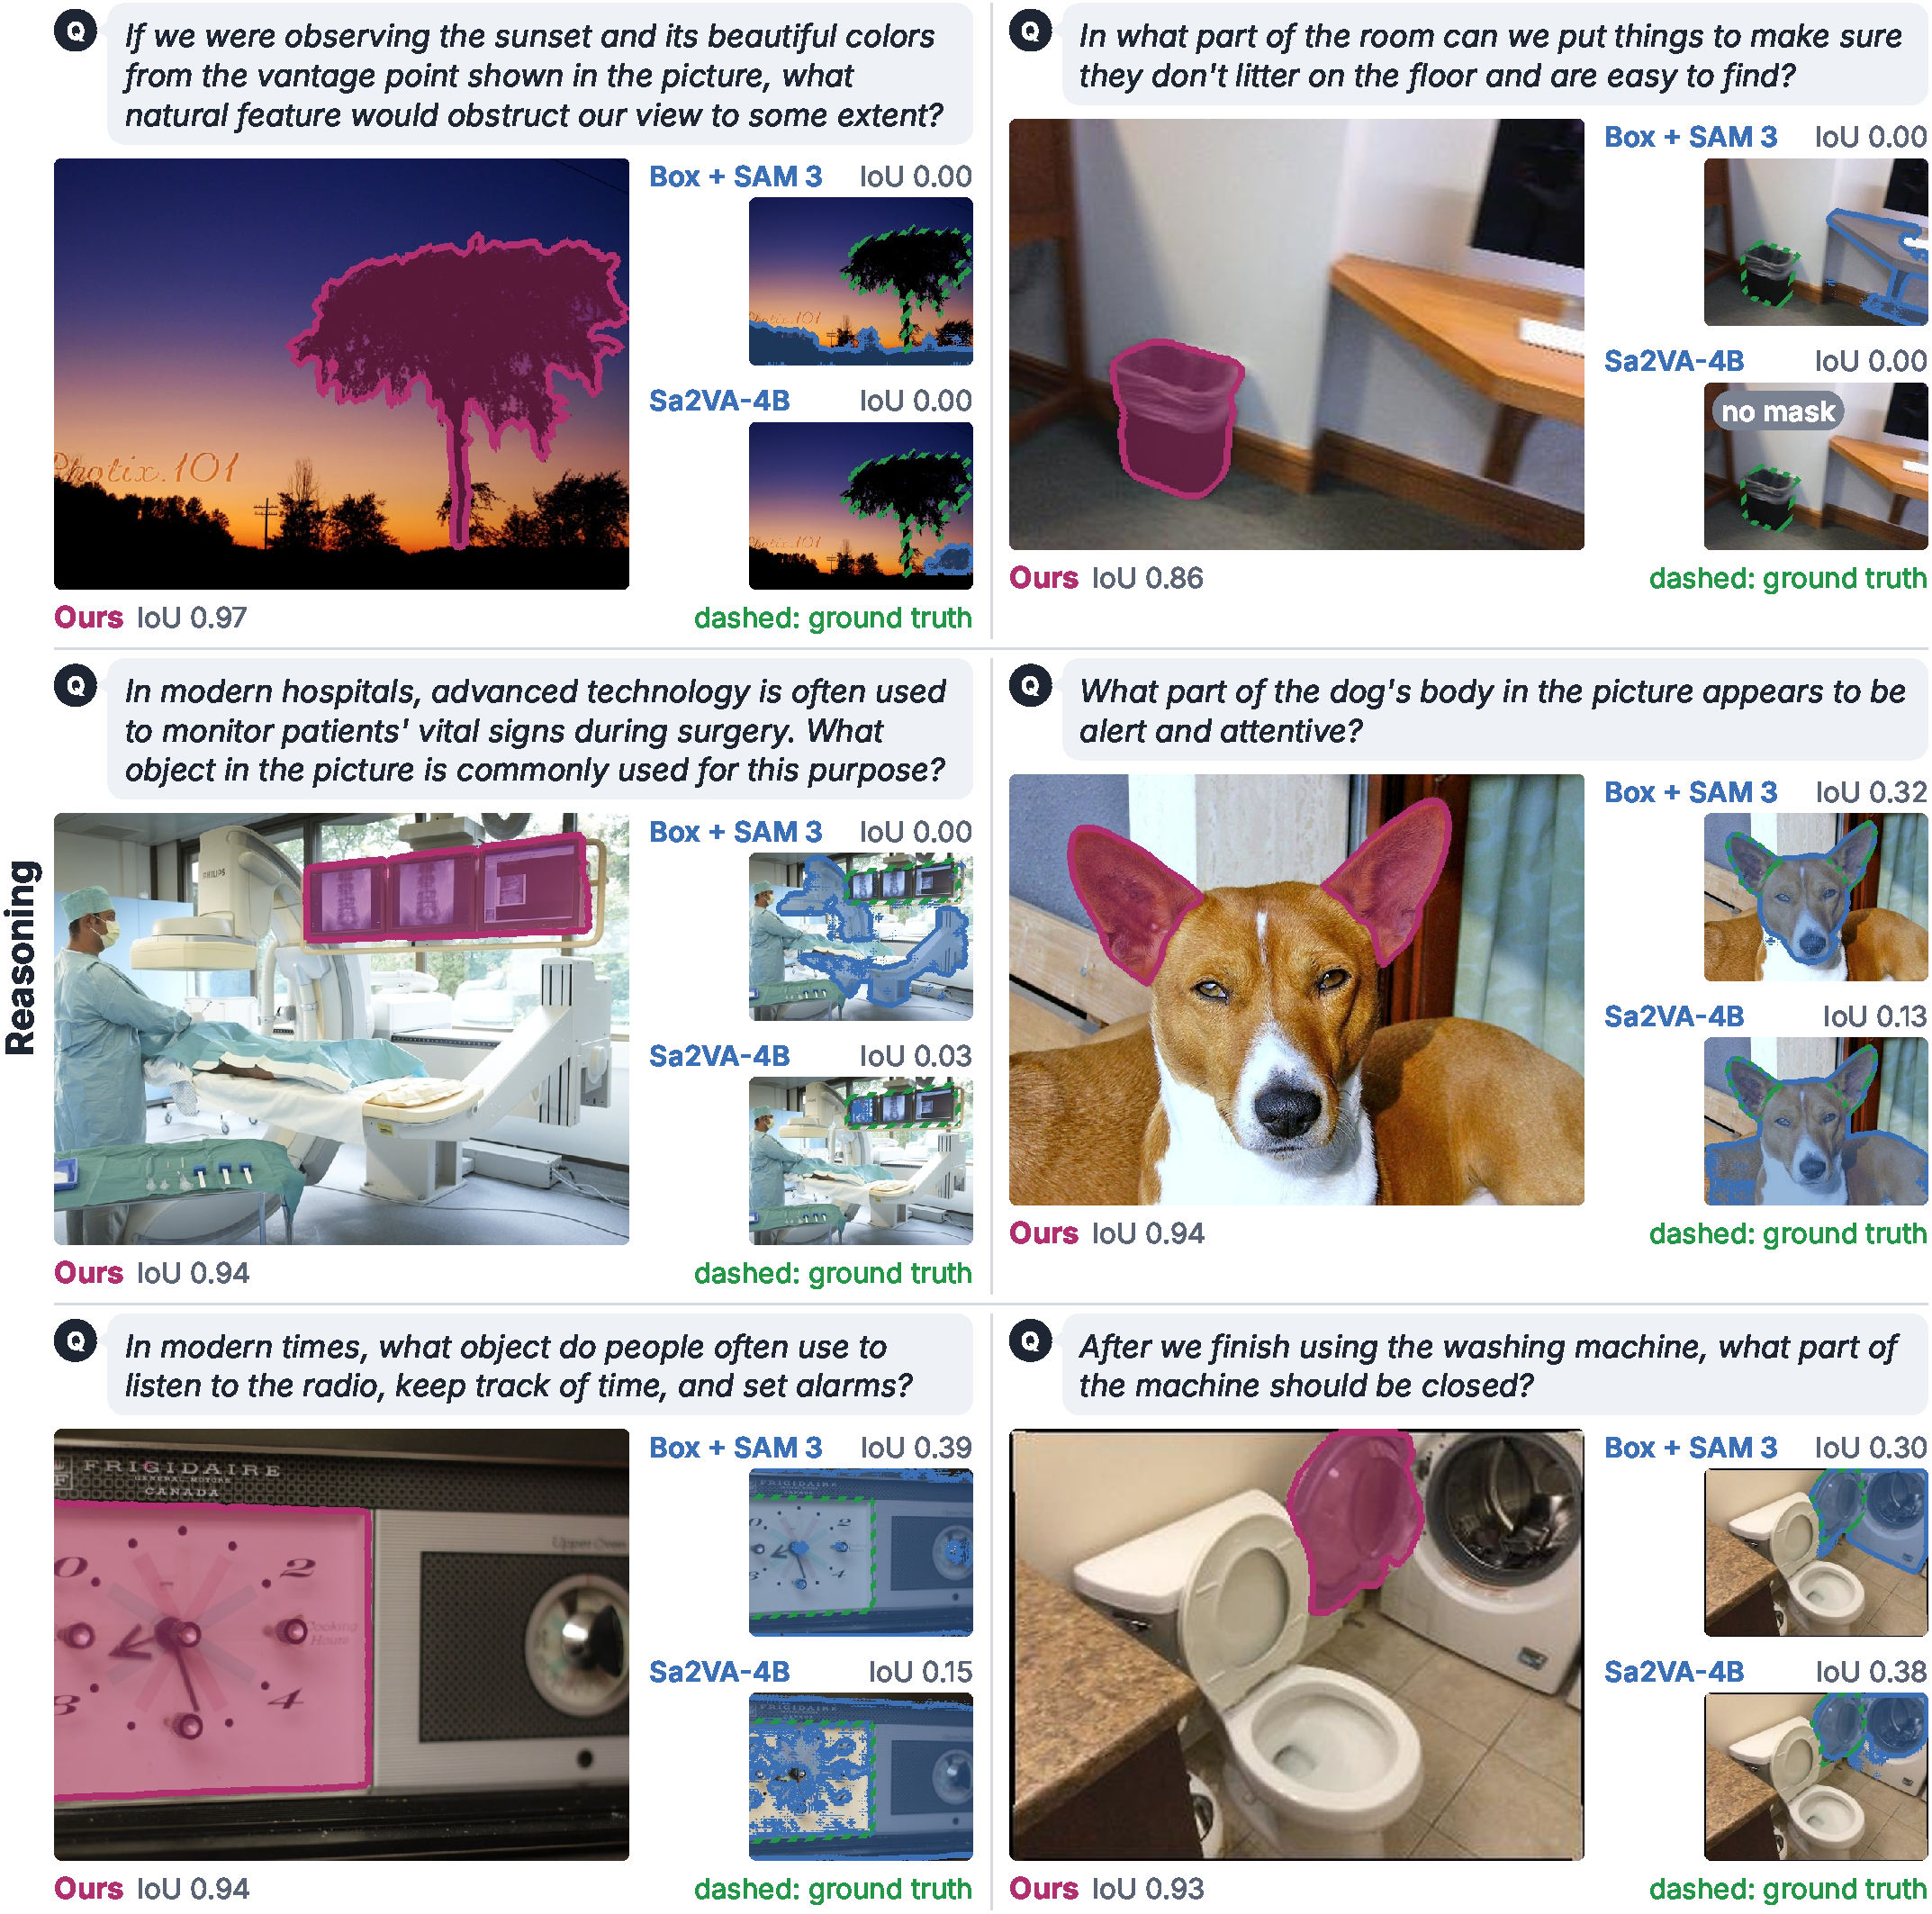
\includegraphics[width=\textwidth,height=0.9\textheight,keepaspectratio]{figures/qualitative/supp/reason_selected_3.pdf}
\caption{\textbf{Reasoning: selected examples (3/3).} Test examples where \ours{} clearly beats Box + SAM\,3, in the format of Fig.~\ref{fig:showcase}; none of them appears in the main paper. Selected examples use query rewriting; random examples and failure cases show \ours{} without it.}
\label{fig:supp_reason_selected_3}
\end{figure*}

\begin{figure*}[p]
\centering
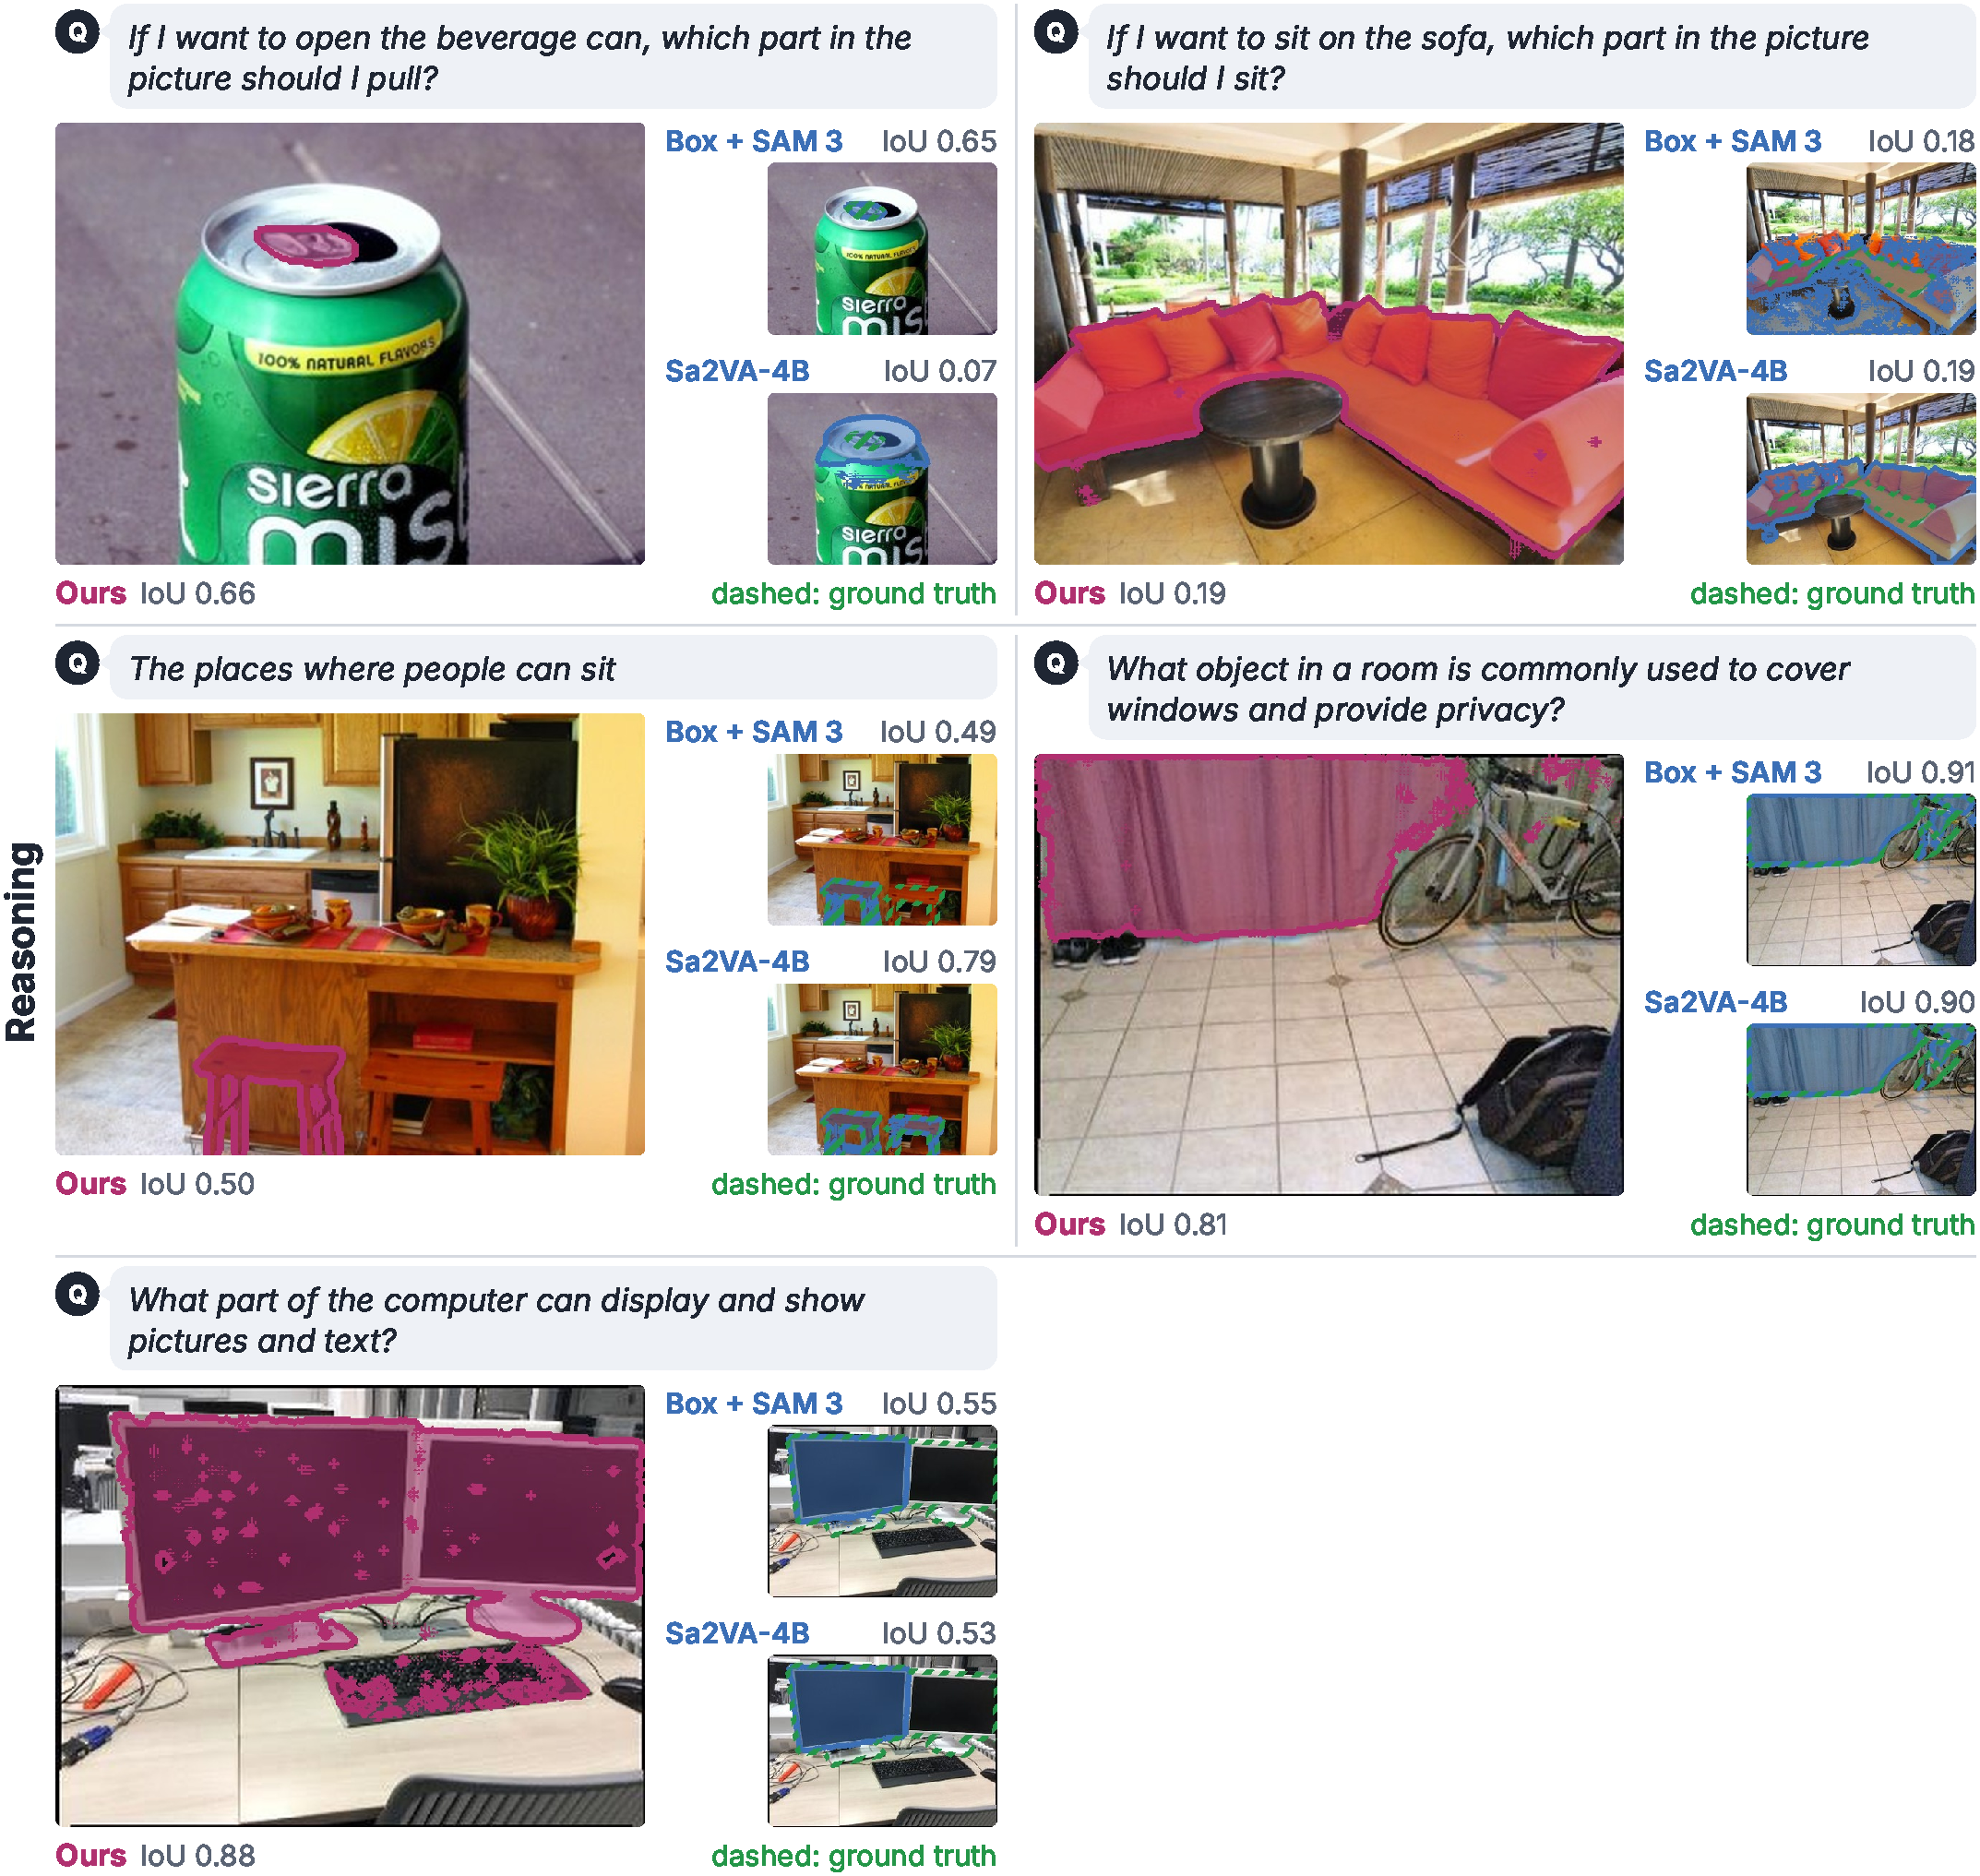
\includegraphics[width=\textwidth,height=0.9\textheight,keepaspectratio]{figures/qualitative/supp/reason_random.pdf}
\caption{\textbf{Reasoning: random examples.} A fixed-seed random sample of test queries, not selected for outcome. Selected examples use query rewriting; random examples and failure cases show \ours{} without it.}
\label{fig:supp_reason_random}
\end{figure*}

\begin{figure*}[p]
\centering
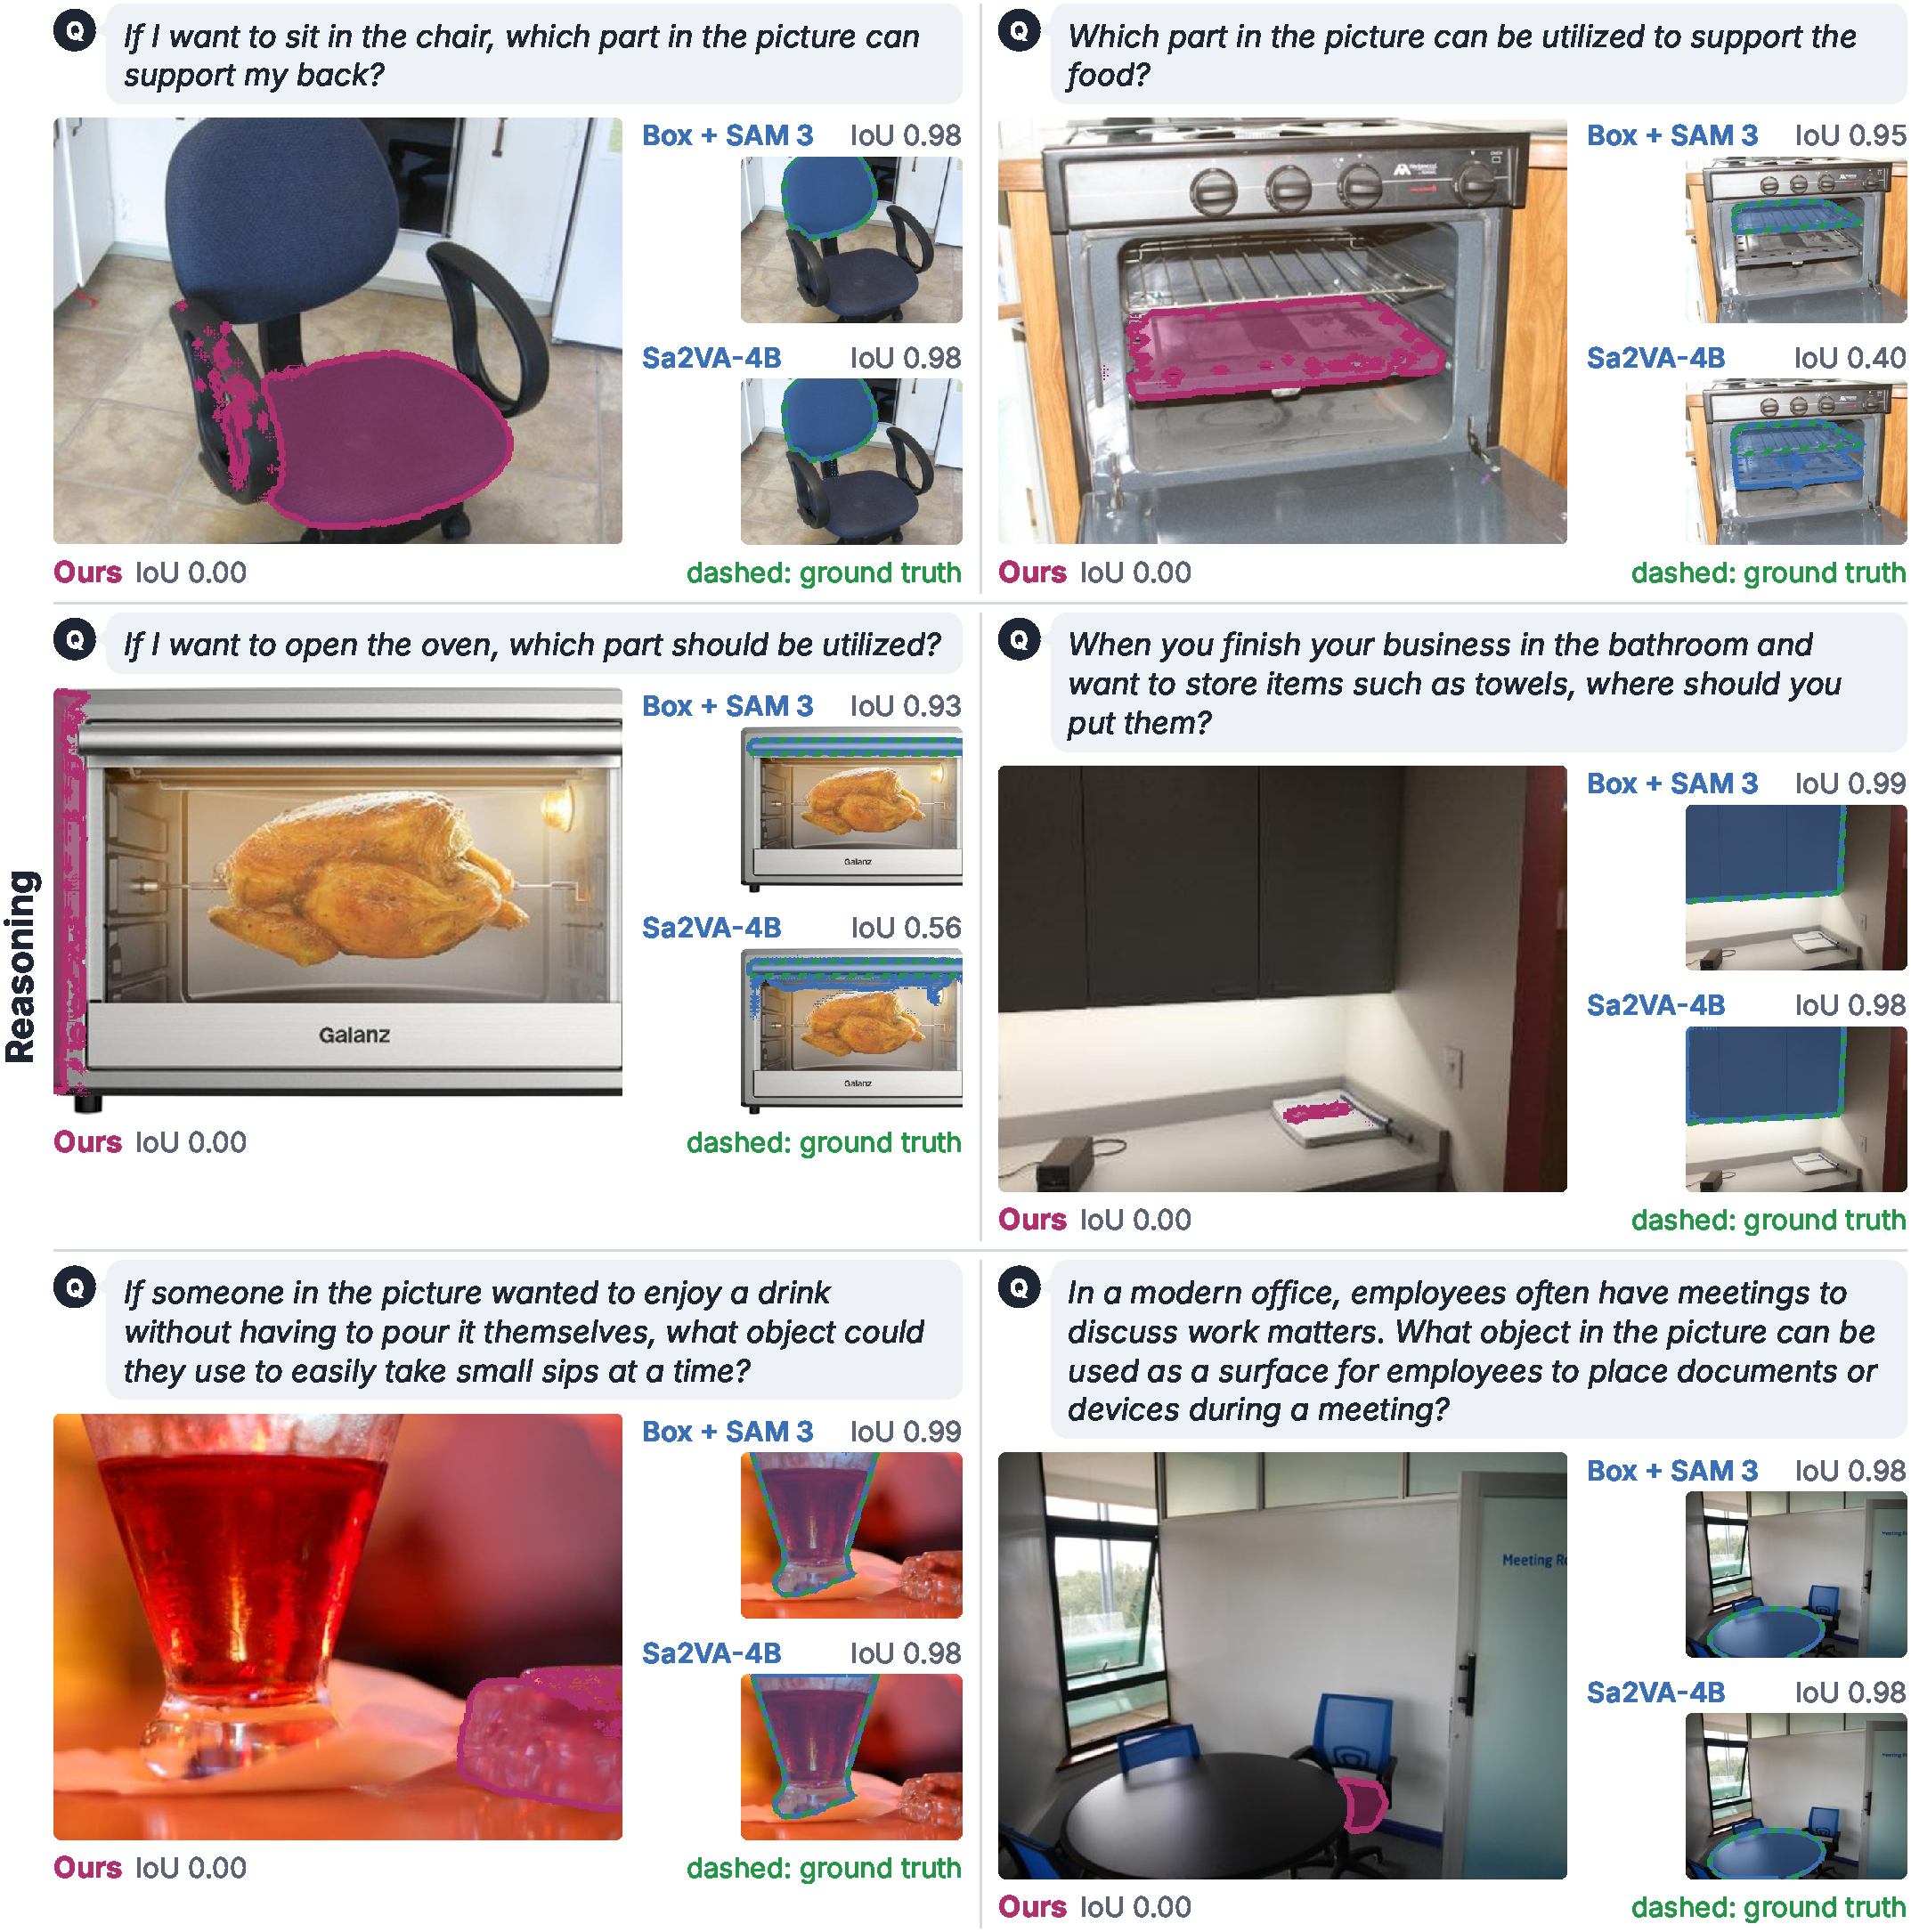
\includegraphics[width=\textwidth,height=0.9\textheight,keepaspectratio]{figures/qualitative/supp/reason_failures.pdf}
\caption{\textbf{Reasoning: failure cases.} The test queries where \ours{} falls furthest behind Box + SAM\,3. Selected examples use query rewriting; random examples and failure cases show \ours{} without it.}
\label{fig:supp_reason_failures}
\end{figure*}

\begin{figure*}[p]
\centering
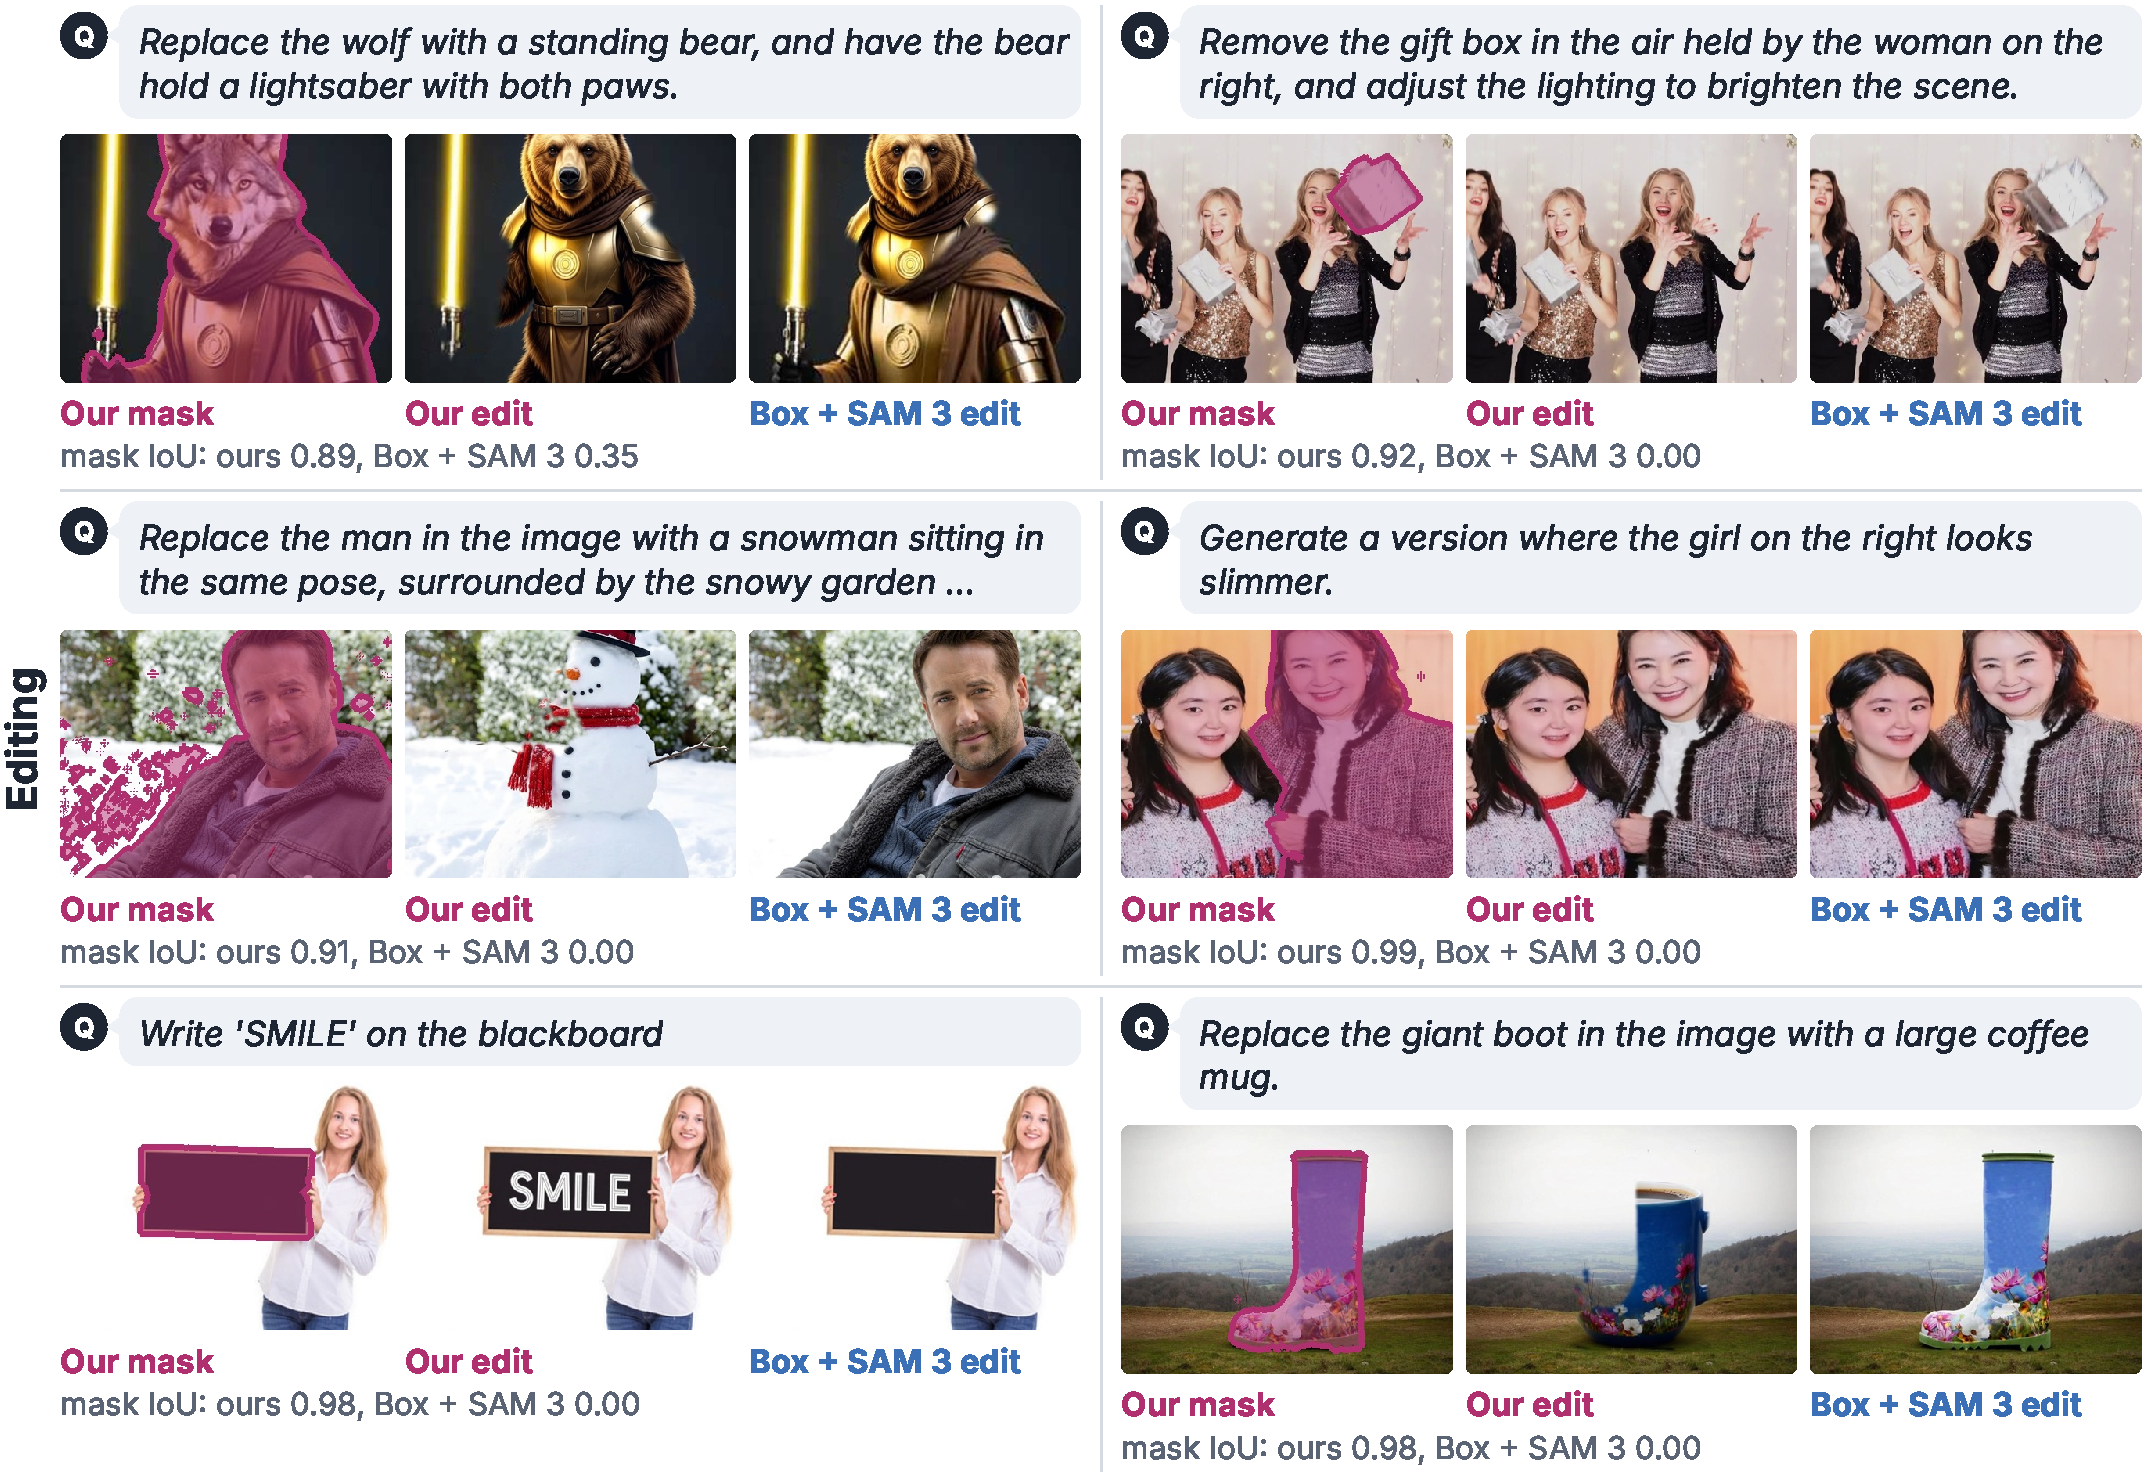
\includegraphics[width=\textwidth,height=0.9\textheight,keepaspectratio]{figures/qualitative/supp/edit_selected_1.pdf}
\caption{\textbf{Editing: selected examples.} Test examples where \ours{} clearly beats Box + SAM\,3, in the format of Fig.~\ref{fig:showcase}; none of them appears in the main paper. Our mask, the edit made with it, and the edit made with the Box + SAM\,3 mask (Qwen-Image-Edit).}
\label{fig:supp_edit_selected_1}
\end{figure*}

\begin{figure*}[p]
\centering
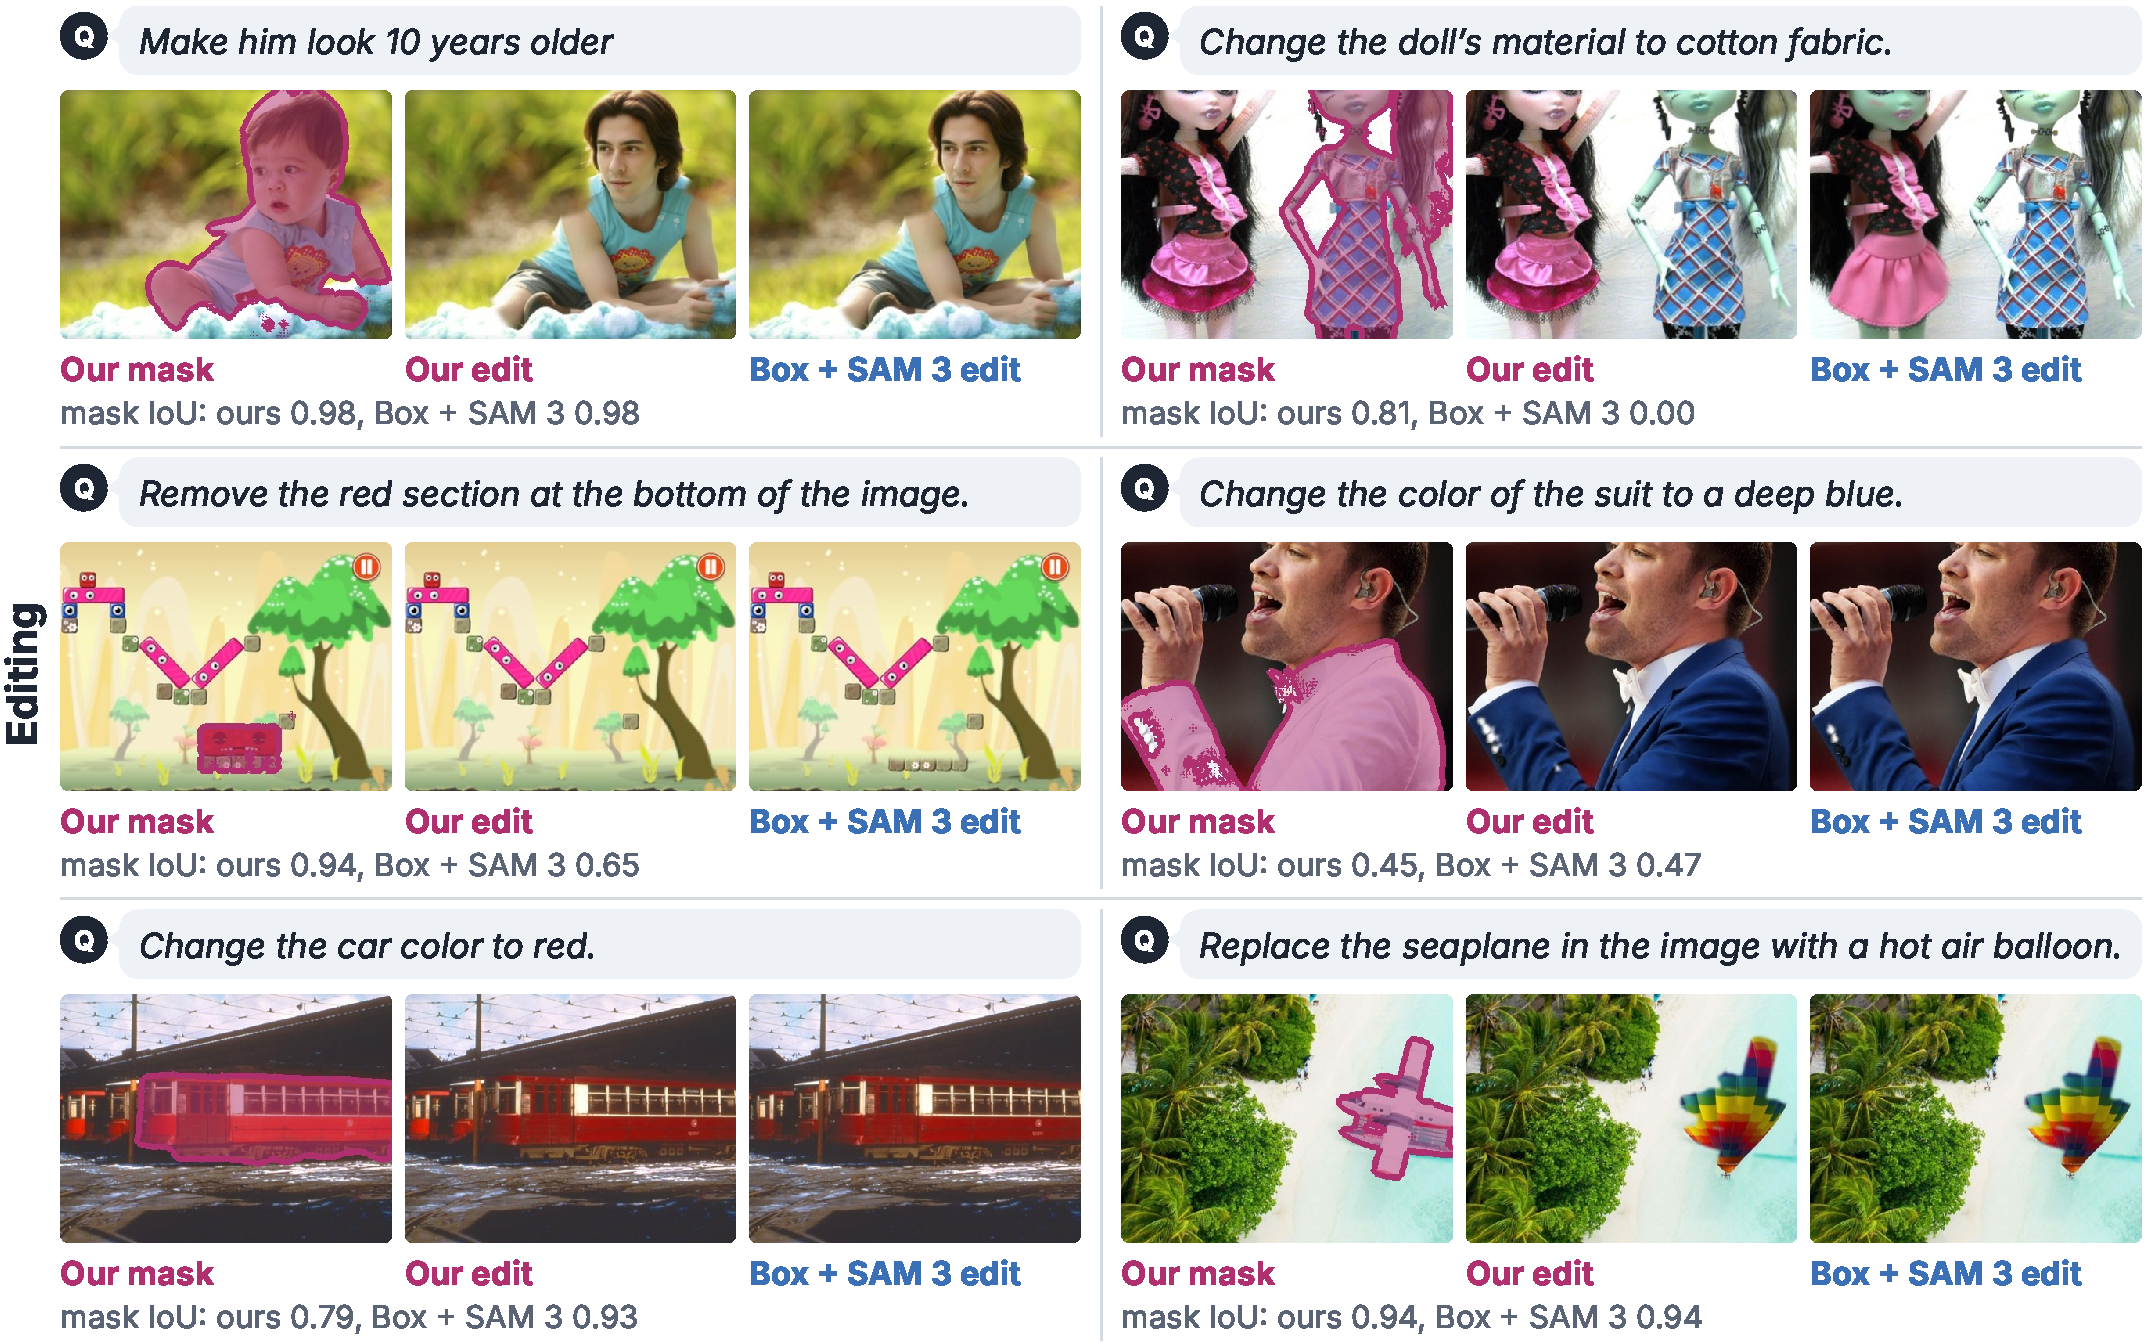
\includegraphics[width=\textwidth,height=0.9\textheight,keepaspectratio]{figures/qualitative/supp/edit_random.pdf}
\caption{\textbf{Editing: random examples.} A fixed-seed random sample of test queries, not selected for outcome. Our mask, the edit made with it, and the edit made with the Box + SAM\,3 mask (Qwen-Image-Edit).}
\label{fig:supp_edit_random}
\end{figure*}

\begin{figure*}[p]
\centering
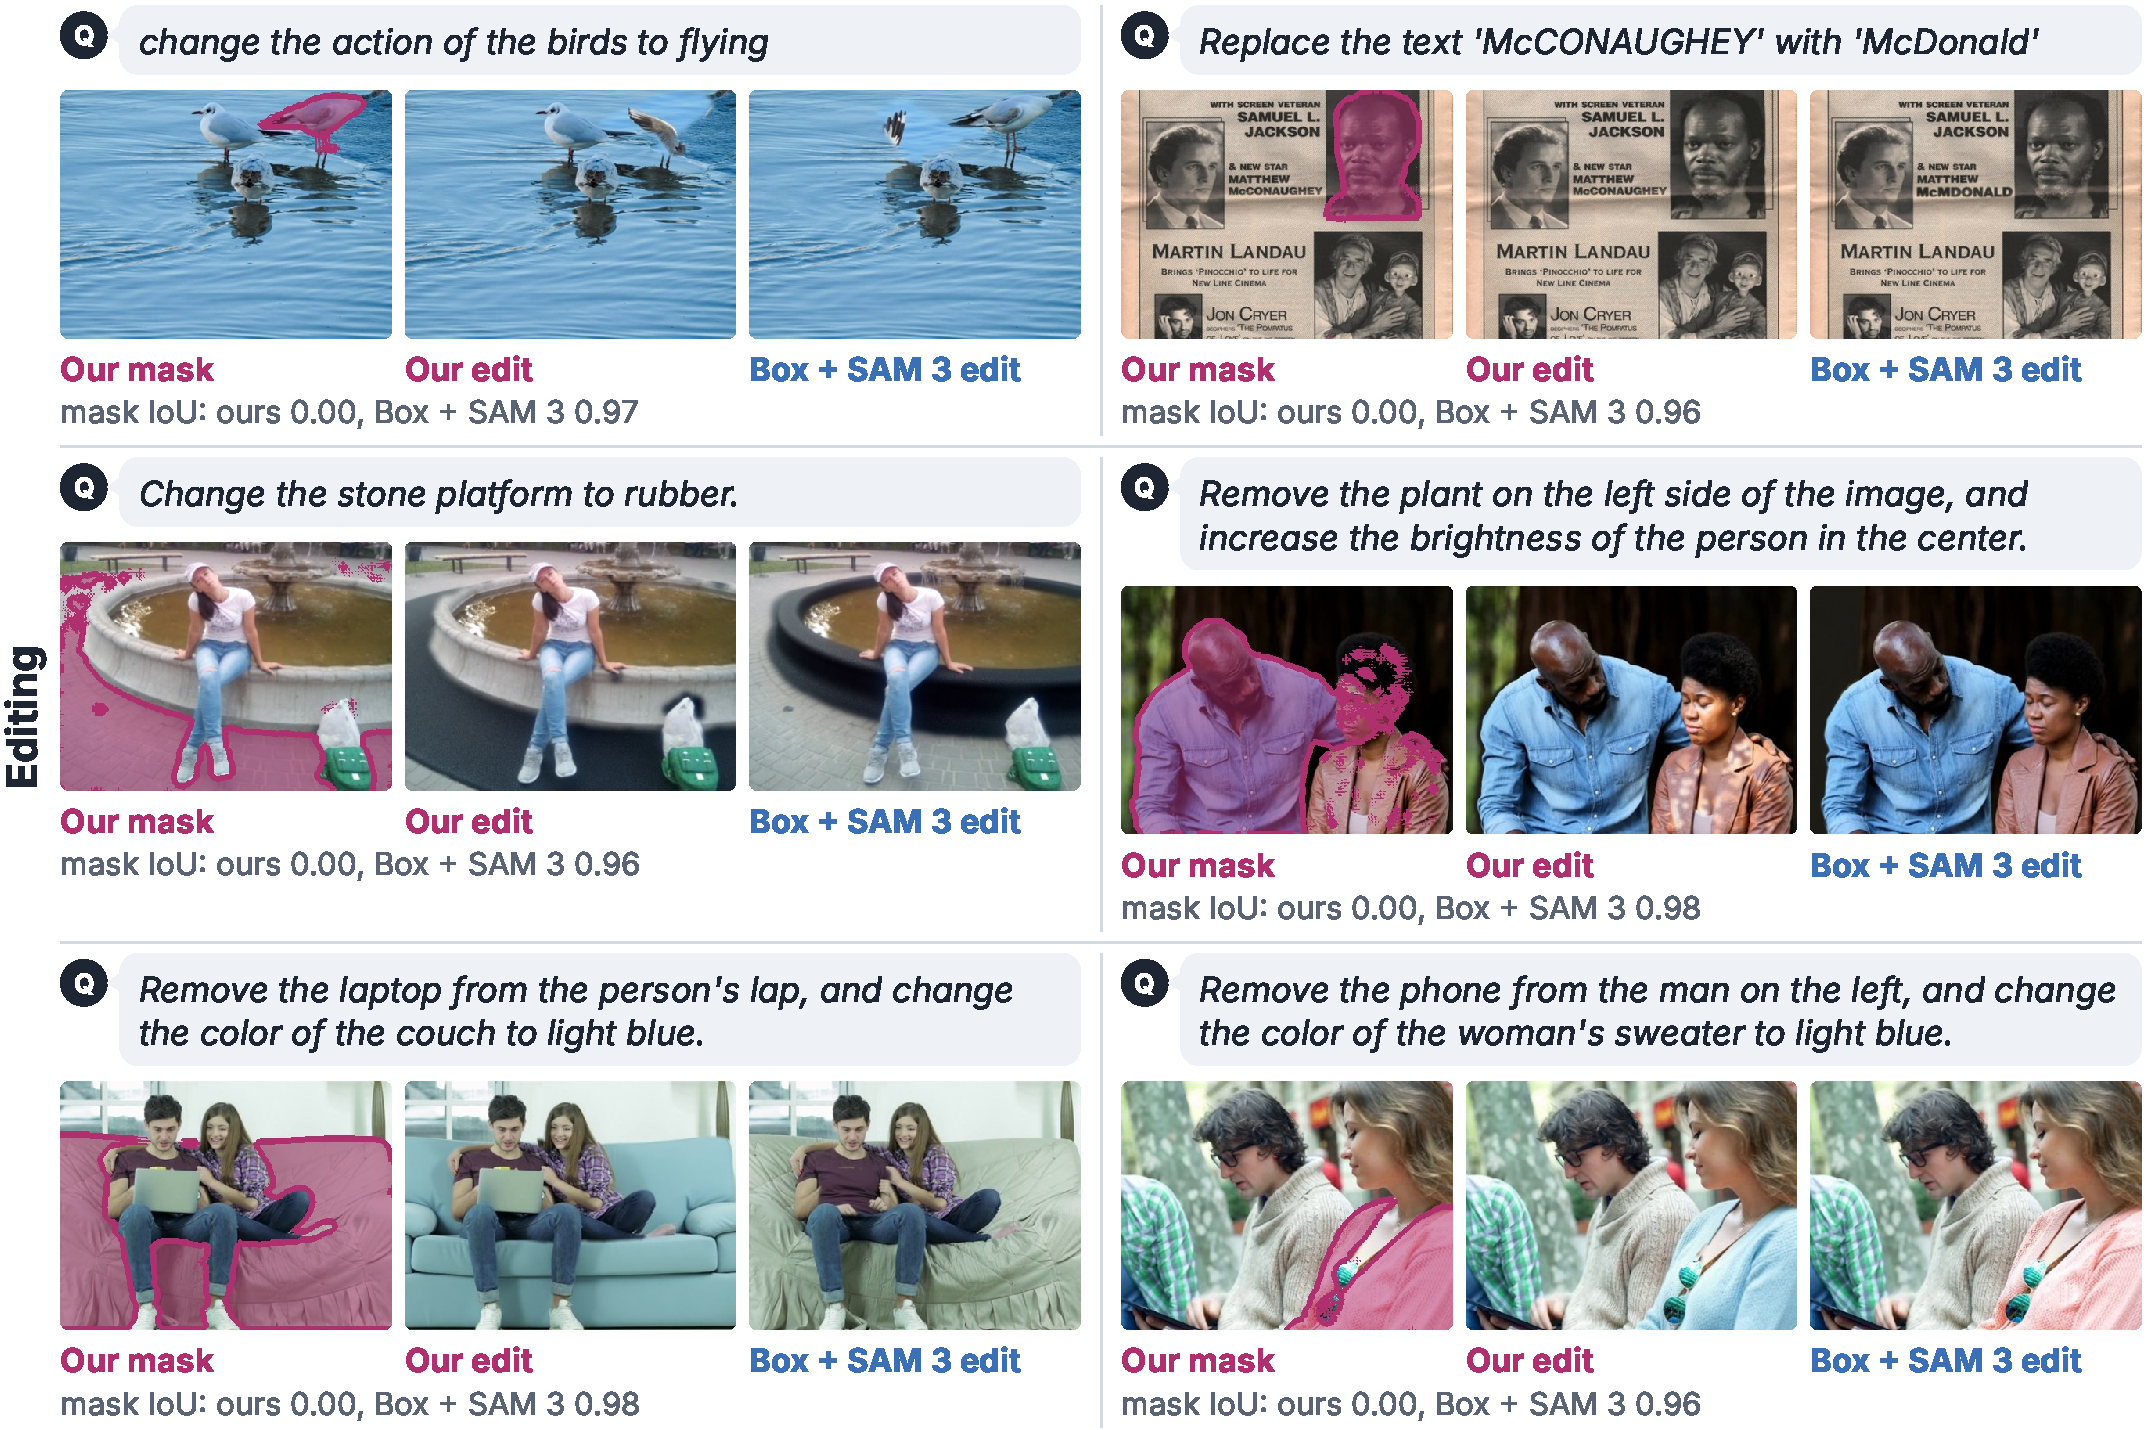
\includegraphics[width=\textwidth,height=0.9\textheight,keepaspectratio]{figures/qualitative/supp/edit_failures.pdf}
\caption{\textbf{Editing: failure cases.} The test queries where \ours{} falls furthest behind Box + SAM\,3. Our mask, the edit made with it, and the edit made with the Box + SAM\,3 mask (Qwen-Image-Edit).}
\label{fig:supp_edit_failures}
\end{figure*}
